\documentclass[apj]{emulateapj}
\usepackage{times}
%\newcommand{\mdot}{M$_{\odot}$\,}
\usepackage{natbib}

\usepackage[backref,breaklinks,colorlinks,citecolor=cyan]{hyperref} 
%\setlength{\parindent}{0pt}
\usepackage{booktabs}
\usepackage{graphicx}
\usepackage{bm}
%\usepackage{deluxetable}
\usepackage{multirow}
\usepackage{enumitem}
\usepackage{amsmath}

\shorttitle{ShortTitle}
\shortauthors{X. Ding et al.}

\begin{document}

\def\lcdm{$\Lambda$CDM}
\def\hst{{\it HST}}
\def\efr{$R_{\mathrm{eff}}$}
\def\galfit{\sc Galfit}
\def\mbh{$\mathcal M_{\rm BH}$}
\def\lhost{$L_{\rm host}$}
\def\jcap{Journal of Cosmology and Astroparticle Physics}
\def\halpha{${\it H}\alpha$}
\def\hbeta{${\it H}\beta$}
\def\sersic{S\'ersic}
\def\lenstronomy{{\sc Lenstronomy}}
\def\Reff{{$R_{\mathrm{eff}}$}}
\def\kms{km~s$^{\rm -1}$}


\title{QSO decomposition}

\author{Xuheng Ding\altaffilmark{1, 2}, Tommaso Treu\altaffilmark{2}, John Silverman\altaffilmark{5}, Simon Birrer\altaffilmark{3}, Malte Schramm\altaffilmark{2}, Federica, Angelea
 }
 \email{dxh@astro.ucla.edu}
% Dandan Xu, Giulia, Anupreeta, Chih-Fan, Daniel, Chris, Phil Marshall, Dominique, 

\altaffiltext{1}{School of Physics and Technology, Wuhan University, Wuhan 430072, China}
\altaffiltext{2}{Department of Physics and Astronomy, University of California, Los Angeles, CA, 90095-1547, USA}
\altaffiltext{3}{Heidelberg Institute for Theoretical Studies, Schloss-Wolfsbrunnenweg 35, D-69118 Heidelberg, Germany}
\altaffiltext{4}{Department of Physics, University of California, Davis, CA 95616, USA}
\altaffiltext{5}{Kavli IPMU (WPI), UTIAS, The University of Tokyo, Kashiwa, Chiba 277-8583, Japan}

\begin{abstract}
To be written. To be written. To be written. To be written. To be written. To be written. To be written. To be written. To be written. To be written. To be written. To be written. To be written. To be written. To be written. To be written. To be written. To be written. To be written. To be written. To be written. To be written. To be written. To be written. To be written. To be written. To be written. To be written. To be written. To be written. To be written. To be written. To be written. 
\end{abstract}

\keywords{galaxies: active --- galaxies: evolution}

\section{Introduction}
\label{sec:introduction}
skeleton of introduction
\\
1. Introduce the ML relation and why understand its evolution is important.\\
2. To understand this evolution, it is important to trace to high redshift. Why it is difficult.\\
3. Introduce reference. Woo's. SS13, Treu's, Park79. In the theory, DeGraf...Highlight the redshift range $z>1.2$\\
4. In this paper, we study the ML relation up to redshift 1.7.

\section{Observations and data reduction}
\label{sec:data}
In this section, we summarize the sample selection, observations, and data reduction of our sample. 

\subsection{Sample selection}
%How the samples are selection.\\
%Where are they from?
%\\The redshift range? In a table?

We aim to study the relation between the BH masses (\mbh) and their host galaxy properties including luminosities (\lhost) and stellar mass to redshift at $z>1$. For this propose, we focus on the broad-line (type-1) AGNs as provided by the X-ray coverage of COSMOS \citep{Civano2016}, (E)-CDFS-S \citep{Lehmer2005, Xue2011}, and SXDS \citep{Ueda2008} fields. We select the broad-line AGNs at redshift region $1.2<z<1.7$ which cover a BH range $7.5<{\rm log}$\mbh $<8.5$. The Near IR spectra of AGNs are available from the survey of Subaru's Fiber Multi-Object Spectrograph \citep[FMOS, ][]{Kimura2010, Schulze2018}, a near-infrared (0.9-1.8 $\mu m$) spectrograph have with 400 apertures. The FMOS survey provides the best \mbh\ estimates by \halpha\ and \hbeta\ lines out to $z\sim1.7$ \citep{Greene2005, Matsuoka2013, Nobuta2012}.

Our final sample is composed of 36  AGNs; 32 of them are new observations by HST/WFC3 \textcolor{red}{\bf (32+4?, the information of these four sample?)}. Table~\ref{tab:objlist} list all the AGN systems analyzed in this work.


To compare with the samples in the literature, we adopt the samples from ... \textcolor{blue}{\bf (H0licow7)}.
For the calibration with the local relation, we introduce the well-defined 19 local AGN measurements \citep{Ben++10, Peterson2004} which defines the zero-point. 

\subsection{Observation and reduction}
\label{observation}
\subsubsection{HST image Observation}
% The QSO surface photometry in IR Channel Filters.\\
The high spatial resolution of the host image is required for the decomposition of the nuclear/host emission and the accurate estimate of the stellar of the host stellar mass. All the new 32 AGN systems were observed with the HST/WFC3 infrared channel, as the HST program GO-15115, PI: John Silverman. We selected to use the filters F125W $(1.2<z<1.44)$ and F140W $(1.44<z<1.7)$ according to the redshift of the targets. This selection could ensure that the broad \halpha line ($4000\AA$) is not present in the bandpass which could contaminate the host emissions due to the broad wings of the PSF.

%Drizzling, background noise...
For the new 32 AGN systems, each target one has six separate exposures with $\sim399s$ (i.e. total exposure time $\sim2394s$). The six exposures for each dither image were combined by the {\sc astrodrizzle} software package, with an output pixel scale of 0\farcs{0642} by setting \texttt{pixfrac} parameter of 0.8 and a \texttt{gaussian} kernel. The other four AGNs in our sample have been observed with WFC3 serendipitously (2 in COSMOS from Kartaltepe (PI); PID: 13657).
The noise level maps of the imaging data are a requirement in the study. The origin of the noise in each pixel is stems from the read noise, background noise and Poisson noise by the astronomical sources themselves. To take them into account, we measure the read noise and background noise level directly from the empty regions of the data. We calculate the effective exposure time in each pixel based on the drizzled \texttt{WHT} array maps to infer the Poisson noise level. To accurately measure the photometry, we also adopt the {\sc photutils} to estimate the background light which could come from both the sky and the detector.

%With 27/36 of our AGNs having rest-frame UV imaging with HST (COSMOS: F814W, PI: Nicholas Scoville; GEMS: F606W+F850LP), we are able to infer the host color and assess the contribution of both the young and old stellar population to the stellar mass budge \textcolor{blue}{citet Gallazzi+Bell 2009}. 

With 18/32 of our sample have rest-frame UV images by \textcolor{blue}{Scoville, et al. 2007} %arxiv: 0702359}.
Images were taken through the wide ACS/F814W filter at four dither pointing with $507s$ exposures. The final image is drizzled to 0\farcs{03} pixel scale. Given the multi-band image for these systems, we are able to infer their host color and assess the contribution of both the young and old stellar population to the stellar mass budge \textcolor{blue}{citet Gallazzi+Bell 2009} which insures an accurate inference of rest-frame R-band luminosity by K-correction, stellar mass and star formation rate (SFR). 

\subsubsection{AGN Emission Line}
\label{sec:bh_mass}
% The introduction of the BH inferred by the board emission line.
The \mbh\ of type-1 AGNs can be inferred using the so-called virial method. The kinematics of the broad-line region trace the gravitational field of the central black hole, assuming the motion of the broad-line region (BLR) gas is virialised. In this scenario, the width of the emission-line provide the scale of the velocity, while the AGN continuum luminosity establish an empirical scale of the BLR size. The virial method builds on these reverberation mapping results and is directly calibrated to the \mbh.

For our targets, the \halpha\ and \hbeta\ emission-line properties have been investigated by \citet{Schulze2018} using the multi-object spectrograph Subaru/FMOS. We referred to this paper for the details of continuum fitting and emission line modeling. Since the other compared AGNs in the literature used different calibrations of the virial method, we adopt the list of consistent recipes \textcolor{blue}{McGill et al. (2008), H0licow7} to cross-calibrate the \mbh\ for all the samples in order to avoid any systematic bias in Section~\ref{mbh}.
 
\section{Analysis}
\label{sec:Analysis}

\subsection{Surface Photometry}
\subsubsection{PSF library}    
\label{sec:psf_library}
%Introduce the PSF library
The knowledge of the PSF is crucial for this study, especially when the nuclear image is unresolved with light distributed as the point source. Moreover, the PSF in known to be vary according to their frame position and the intensity. Thus, we build a library of PSFs which we select the bright, isolated, unsaturated PSF stars across all the observed field. Thanks to the available multi-wavelength data \textcolor{blue}{(Laigle et al. 2016)}, we are able to know the positions of stars nearby the QSO field and thus select a proper position and orientation of the HST frame to cover as much PSFs stars as possible. 

We claim that, by building this library, the assumption is that the overall PSFs herein indicates all the possible PSF shape for each QSO. Since two filter, i.e. F140W and F125W, are selected for different samples, we selected 74 and 34 PSFs for the samples observed by F140W and F125W, respectively.

In the next subsection, we carry out the QSO decomposition using each PSF. We rank their performance based on the goodness so that the final inference of the host properties are weighted from the top-rank PSFs.

\subsubsection{Surface Photometry modeling method}
%Introduce the lenstronomy. Model the PSF in each library.\\
%Inspired by Simon's work, we rank the performance of the each PSF and weight for the final fitting result. 
We simultaneously fit the two-dimensional flux distribution of the center nuclear and the underling host galaxy. Following common practice, we assume the unresolved nuclear as a scaled PSF image, while the host galaxy as a \sersic\ profile. Note that the actual morphologies of the host galaxies could be even more complicated (e.g. bulge+disk). However, the purpose of adopting the \sersic\ model is a simplified a first-order approximation of the surface brightness distribution with a flexible parameterization which provides sufficient freedom to infer the host flux given the high redshift range of our sample. We fit the objects which close to the QSO as the another \sersic\ model, to minimize the impact of their light.

%Introduce Lenstronomy:
We adopt the imaging modeling tool \lenstronomy\ \textcolor{blue}{(arXiv:1803.09746)}, to decompose the host and nuclear image. The \lenstronomy\ is a multi-purpose open-source gravitational lens modeling python package. 
The flexibility of this package enable us to turn off the lensing channel and carry out the decomposition.
We have tested that the inference by \lenstronomy\ could have consistent result compared to {\sc Galfit}. \textcolor{red}{Will talk more in this part.}

%Introduce the final inference using fitting:
For each QSO system, the final host properties is inferred in several steps. First, we fit the flux distribution using each PSFs in the library. Given the QSO imaging data, PSF and noise level, we are able to infer the posterior distribution in the parameter space and optimize the best-fit parameters with minimized residuals. In this step, we infer the best-fit parameters for each PSFs in the library and the corresponding $\chi^2$ value\footnote{The \lenstronomy\ enable one to infer also the parametric confidence interval. However, given a fixed PSF image, the $1-\sigma$ region of each parameter are extremely narrow}. In the second step, we rank the performance of each PSF based on the reduced $\chi^2$ value and select the top-8 PSFs so as to weight for the inferred property. The weights for each PSF is calculated by:
\begin{eqnarray}
\label{eq:weights}
w_i = exp \big(-\frac{ (\chi_i ^2 - \chi_{best} ^2 )}{2\alpha \chi_{best} ^2} \big),
\end{eqnarray} 
where the $\alpha$ is the inflation parameter so that when $i=8$:
\begin{eqnarray}
\label{eq:alpha}
\alpha \frac{ \chi_{i=8} ^2 - \chi_{best} ^2 }{2 \chi_{best} ^2} = 2
\end{eqnarray} 

%ECDFS-358 and CID206

In Figure~\ref{fig:QSO_decomp}, we demonstrate the optimized result of each system inferred by \lenstronomy. We also show the weighting process for an example system -- CID1174 in Table~\ref{tab:weight_CID1174}. In Figure~\ref{fig:flux_r_n_corner}, we summarize the relation among the inferred values of: \Reff, \sersic\ $n$, and host to total flux ratio. 

%The inference of F814w data.
Likewise, for the 18 systems with ACS/F184W images, we infer their host properties using the same approach. There are in total 174 star-like PSFs in the fitting library. We assumed the shape of the galaxy are consistent between the ACS and WFC3. Since the effects of dust extinction and contrast between the (blue) AGN and (red) host is more favorable in IR band, we believe the inferred information of the galaxy shape by IR band are superior to the one by UV band. Thus, while fitting the host flux at ACS band, we fix the \Reff\ and \sersic\ $n$ to the value by IR.

We list all the inference of the host galaxy properties in the Table~\ref{tab:result_sersic}.

%The overall fitting plot: 1. Host-R-n corner for f140w and f814w. 2. The histogram with different selection.

\subsubsection{Host luminosity}
\textcolor{red}{To be written:}
1.K-correction to infer the rest frame R-band.\\
* The galaxy template inferred by the joint fitting of the SED and the host flux ratio by us.

Having inferred the value of the rest-frame R-band magnitude, the luminosity is derived by $\log L_R/L_{R, \odot} = 0.4 (M_{R, \odot}-M_R)$, where $M_{R, \odot}=4.61$ \citep{Blanton07}.

\textcolor{blue}{Introduce the passive evolution?}
To directly compare with local samples, we consider the passive evolution scenario for the inferred \lhost\ and transfer to its expected value at today.

We summarized the homogenized R-band luminosities
in Table~\ref{tab:result_sersic}.

\subsection{BH masses}
\label{mbh}
Our selected systems are broad-line (type-1) AGNs whose \mbh\ can be estimated from single-epoch spectroscopy using the so-called virial method \textcolor{blue}{FMOS (e.g. McLure 2002; Shen 2013)}. This estimation is achieved by the assumption that the empirical scaling size of the BLR and the line-of-sight velocity width can be inferred in turn continuum luminosity ($L _{\lambda_{\rm line}}$) and emission line width (FWHM), respectively.

To avoid any systematic bias between our samples and the literature samples, we cross-calibrate the \mbh\ by adopting the self-consistent recipes as used by \textcolor{blue}{H0licow7, McGill et al. (2008)}. Overall, we adopt the following virial formalism for the \halpha\ and \hbeta\ emission line:

\begin{eqnarray}
\label{eq:Hb}
\log \left(\frac{\mathcal M_{\rm BH}(H\beta) }{M_{\odot}}\right)&~=~& 6.882+0.518\log \left(\frac{ \lambda \rm L _{\lambda_{5100}}}{10^{44}{\rm erg~s^{-1}}}\right) \nonumber\\
&~+~& 2 \log \left(\frac{\rm FWHM(5100)}{1000 ~{\rm km~s^{-1}}}\right) , 
\end {eqnarray}

and

\begin{eqnarray}
\label{eq:Ha}
\log \left(\frac{\mathcal M_{\rm BH} (H\alpha)}{M_{\odot}}\right)&~=~& 6.459+0.55 \log \left(\frac{ \lambda \rm L _{H\alpha}}{10^{42}{\rm erg~s^{-1}}}\right) \nonumber\\
&~+~& 2 \log \left(\frac{\rm FWHM(H\alpha)}{1000 ~{\rm km~s^{-1}}}\right) , 
\end {eqnarray}

Having defined the recipes, we estimate the \mbh\ by adopting the emission line properties measured by \citet{Schulze2018}. 14 of the overall systems have both \halpha\ and \hbeta\ emission line information; we adopt the average \mbh\ value by these two lines. We summarized the inference of the \mbh\ together with the details on the emission line in Table~\ref{tab:result_mbh}.


\section{Results}
\label{sec:result}
\subsection{\mbh-\lhost\ relation}

\subsection{\mbh-M$_*$ relation}
\subsubsection{Stellar mass estimates}
stellar mass \\

\section{Summary}
\label{sec:sum}
We presented the study of the Mbh and host property's evolution to high redshift until 1.8.

\section{discuss}
\label{sec:dis}
\subsection{Systematic error}
\subsection{Fitting mask for CID206 and ECDFS-358}

\section*{Acknowledgments}
We thank the people who discuss with the paper.

\bibliographystyle{apj.bst}
\bibliography{references}

\begin{deluxetable}{llccc}
\tablecolumns{5}
\tablewidth{0pt}
\tablecaption{The sample information for the 32 systems.} 
\tablehead{ 
\colhead{Object ID} &
\colhead{$z$} & 
\colhead{WFC3/Filter} &
\colhead{$RA$}&
\colhead{$DEC$}
 \\ 
\colhead{(1)} &
\colhead{(2)} &
\colhead{(3)} &
\colhead{(4)} &
\colhead{(5)} 
} 
\startdata
%\multicolumn{5}{c}{Sample presented in \citet{Treu+07}}\\
%\\
COSMOS-CID1174 & 1.552 & F140W$^*$ & 150.2789 & 1.9595\\
COSMOS-CID1281 & 1.445 & ??? & 150.4160 & 2.5258\\
COSMOS-CID206 & 1.483 & F140W & 149.8371 & 2.0088\\
COSMOS-CID216 & 1.567 & F140W$^*$ & 149.7918 & 1.8729\\
COSMOS-CID237 & 1.618 & F140W$^*$ & 149.9916 & 1.7243\\
COSMOS-CID255 & 1.664 & ???$^*$ & 150.1017 & 1.8483\\
COSMOS-CID3242 & 1.532 & F140W & 149.7113 & 2.1452\\
COSMOS-CID3570 & 1.244 & F125W & 149.6411 & 2.1076\\
COSMOS-CID452 & 1.407 & F125W$^*$ & 150.0045 & 2.2371\\
COSMOS-CID454 & 1.478 & F140W$^*$ & 149.8681 & 2.3307\\
COSMOS-CID50 & 1.239 & F125W$^*$ & 150.2080 & 2.0833\\
COSMOS-CID543 & 1.301 & F125W$^*$ & 150.4519 & 2.1448\\
COSMOS-CID597 & 1.272 & ???$^*$ & 150.5262 & 2.2449\\
COSMOS-CID607 & 1.294 & F125W$^*$ & 150.6097 & 2.3231\\
COSMOS-CID70 & 1.667 & F140W & 150.4051 & 2.2701\\
COSMOS-LID1273 & 1.617 & F140W & 150.0565 & 1.6275\\
COSMOS-LID1538 & 1.527 & F140W$^*$ & 150.6215 & 2.1588\\
COSMOS-LID360 & 1.579 & F140W$^*$ & 150.1251 & 2.8617\\
COSMOS-XID2138 & 1.551 & F140W$^*$ & 149.7036 & 2.5781\\
COSMOS-XID2202 & 1.516 & F140W$^*$ & 150.6530 & 1.9969\\
COSMOS-XID2396 & 1.600 & F140W$^*$ & 149.4779 & 2.6425\\
CDFS-1 & 1.630 & F140W$^*$ & 52.8990 & -27.8600\\ 
CDFS-229 & 1.326 & F125W$^*$ & 53.0680 & -27.6580\\ 
CDFS-321 & 1.570 & F140W$^*$ & 53.0486 & -27.6239\\ 
CDFS-724 & 1.337 & F125W & 53.2870 & -27.6940\\ 
ECDFS-358 & 1.626 & F140W & 53.0850 & -28.0370\\ 
SXDS-X1136 & 1.325 & F125W & 34.8925 & -5.1498\\ 
SXDS-X50 & 1.411 & F125W & 34.0267 & -5.0602\\ 
SXDS-X717 & 1.276 & F125W & 34.5400 & -5.0334\\ 
SXDS-X735 & 1.447 & F140W & 34.5581 & -4.8781\\ 
SXDS-X763 & 1.412 & F125W & 34.5849 & -4.7864\\ 
SXDS-X969 & 1.585 & F140W & 34.7594 & -5.4291\\ 
\enddata
\label{tab:objlist}
\tablecomments{
Column 1: Object field and ID.
Column 2: Redshifts.
Column 3: HST filter by WFC3. The marker $^*$ indicate the corresponding sample also has the ACS/F814W image.
Column 4 and 5: The $RA$ and $DEC$ of the system.
}
\end{deluxetable}

\begin{deluxetable*}{ccccccc}
\tablecolumns{7}
\tablewidth{0pt}
\tablecaption{Details of the weighting CID1174's inference. } 
\tablehead{ 
\colhead{PSF rank} &
\colhead{total $\chi ^2$} & 
\colhead{weights $w_i$} &
\colhead{host flux (counts)} &
\colhead{host flux ratio}&
\colhead{\Reff (arcsec)}&
\colhead{\sersic\ $n$}
 \\ 
\colhead{(1)} &
\colhead{(2)} &
\colhead{(3)} &
\colhead{(4)} &
\colhead{(5)} &
\colhead{(6)} &
\colhead{(7)} 
} 
\startdata
%\multicolumn{5}{c}{Sample presented in \citet{Treu+07}}\\
%\\
1 & 8646.711 & 1.000 & 99.102 & 41.9\% & 0\farcs{}298 & 1.932 \\
2 & 8816.947 & 0.849 & 76.740 & 33.0\% & 0\farcs{}365 & 1.102 \\
3 & 9304.841 & 0.530 & 128.618 & 54.7\% & 0\farcs{}231 & 2.780 \\
4 & 9652.575 & 0.379 & 187.498 & 79.0\% & 0\farcs{}116 & 6.175 \\
5 & 10018.324 & 0.267 & 75.061 & 32.3\%& 0\farcs{}365 & 1.226 \\
6 & 10087.456 & 0.249 & 79.835 & 34.3\% & 0\farcs{}358 & 1.195 \\
7 & 10457.811 & 0.174 & 108.580 & 46.4\% & 0\farcs{}262 & 2.190 \\
8 & 10721.421 & 0.135 & 63.994 & 27.8\% & 0\farcs{}406 & 0.720 \\
\hline\\
Weighted value & & & 103.534 $\pm$ 34.267 & 44.0\%$\pm$14.2\%& 0\farcs{}296$\pm$0\farcs{}079 & 2.173$\pm$1.500  \\
\enddata
\label{tab:weight_CID1174}
\tablecomments{
Column~1: The rank of the PSF from the library.
Column~2: Total $\chi ^2$ for the corresponding PSF.
Column~3: Weights for co-adding the inference.
Column~4-7: Fitted value for the host flux, host/total flux ratio, effective radius, and \sersic\ index.
For this sample, the inflation value $\alpha$ calculated by Eq.~\ref{eq:alpha} is 16.671.
}
\end{deluxetable*}

\begin{deluxetable*}
{@{\extracolsep{4pt}}lccccccccc}   % need for the gap between the clines.
\tablecolumns{9}
\tablewidth{0pt}
\tablecaption{The inference of the host information by the QSO decomposition for the 32 systems.} 
\tablehead
{ 
\colhead{Target ID}&
  \multicolumn{5}{c}{Inference by WFC3}&
  \multicolumn{3}{c}{Inference by ACS} \\
  \cline{2-6}  \cline{7-9} \\
\colhead{}& 
\colhead{reduced $\chi ^2$}& \colhead{host flux ratio}& 
\colhead{\Reff}& \colhead{\sersic\ $n$}& 
\colhead{magnitude}&
\colhead{reduced $\chi ^2$}& \colhead{host flux ratio}& \colhead{magnitude} & \colhead{$\log L_R$}\\
\colhead{}& 
\colhead{}& \colhead{}& 
\colhead{($\arcsec$)}& \colhead{}& 
\colhead{(AB system)}& \colhead{}& 
\colhead{}& \colhead{(AB system)}&\colhead{($L_{\odot,R}$)} \\
\colhead{(1)}& 
\colhead{(2)}& \colhead{(3)}& 
\colhead{(4)}& \colhead{(5)}& 
\colhead{(6)}& \colhead{(7)}& 
\colhead{(8)}& \colhead{(9)}&\colhead{(10)}
}
\startdata 
CID1174 & 2.324 & 44.0\%$\pm$14.2\% & 0.296$\pm$0.079 & 2.173$\pm$1.5 & $21.415\substack{+0.436 \\ -0.31}$ & 2.484074 & 11.7\%$\pm$1.4\% & $23.165\substack{+0.138 \\ -0.122}$\\
CID1281 & ... & ... & ... & ... & ... & ... & ... & ...\\
CID206 & 2.054 & 35.7\%$\pm$24.1\% & 0.282$\pm$0.151 & 3.191$\pm$2.51 & $21.81\substack{+1.247 \\ -0.565}$ & 1.903449 & 7.7\%$\pm$2.4\% & $23.671\substack{+0.403 \\ -0.293}$\\
CID216 & 1.514 & 93.9\%$\pm$4.7\% & 0.251$\pm$0.063 & 6.159$\pm$1.205 & $21.51\substack{+0.052 \\ -0.049}$ & 1.424993 & 35.1\%$\pm$1.5\% & $23.446\substack{+0.053 \\ -0.051}$\\
CID237 & 2.349 & 29.9\%$\pm$6.3\% & 0.872$\pm$0.172 & 4.736$\pm$1.701 & $21.279\substack{+0.26 \\ -0.209}$ & 2.353571 & 3.2\%$\pm$2.0\% & $23.718\substack{+1.037 \\ -0.52}$\\
CID255 & ... & ... & ... & ... & ... & ... & ... & ...\\
CID3242 & 2.751 & 46.1\%$\pm$12.7\% & 0.201$\pm$0.159 & 6.142$\pm$1.874 & $21.161\substack{+0.35 \\ -0.264}$ & 2.595594 & 4.8\%$\pm$1.3\% & $23.595\substack{+0.337 \\ -0.257}$\\
CID3570 & 1.665 & 76.5\%$\pm$1.6\% & 0.698$\pm$0.007 & 0.728$\pm$0.054 & $21.164\substack{+0.021 \\ -0.021}$ & 1.331913 & 85.6\%$\pm$1.5\% & $22.971\substack{+0.012 \\ -0.012}$\\
CID452 & 1.684 & 75.4\%$\pm$3.9\% & 0.365$\pm$0.015 & 1.402$\pm$0.175 & $21.176\substack{+0.063 \\ -0.06}$ & 1.451608 & 37.8\%$\pm$0.7\% & $22.732\substack{+0.022 \\ -0.022}$\\
CID454 & 2.203 & 35.3\%$\pm$2.1\% & 0.391$\pm$0.013 & 0.602$\pm$0.092 & $21.212\substack{+0.067 \\ -0.063}$ & 1.29101 & 9.2\%$\pm$0.5\% & $23.352\substack{+0.058 \\ -0.055}$\\
CID50 & 5.576 & 16.8\%$\pm$8.7\% & 0.152$\pm$0.102 & 3.371$\pm$2.154 & $20.915\substack{+0.796 \\ -0.454}$ & 4.940352 & 5.0\%$\pm$3.3\% & $22.504\substack{+1.145 \\ -0.545}$\\
CID543 & 1.902 & 31.8\%$\pm$10.0\% & 0.1$\pm$0.0 & 0.505$\pm$0.333 & $21.95\substack{+0.405 \\ -0.294}$ & 1.434799 & 5.2\%$\pm$2.0\% & $23.765\substack{+0.534 \\ -0.357}$\\
CID597 & ... & ... & ... & ... & ... & ... & ... & ...\\
CID607 & 1.692 & 43.6\%$\pm$17.9\% & 0.206$\pm$0.087 & 3.418$\pm$1.097 & $21.189\substack{+0.575 \\ -0.374}$ & 2.590398 & 4.7\%$\pm$1.8\% & $23.566\substack{+0.511 \\ -0.346}$\\
CID70 & 2.041 & 19.6\%$\pm$5.1\% & 0.426$\pm$0.101 & 3.543$\pm$1.154 & $21.865\substack{+0.323 \\ -0.248}$ & 2.36054 & 2.3\%$\pm$1.1\% & $24.625\substack{+0.677 \\ -0.414}$\\
LID1273 & 1.697 & 53.3\%$\pm$9.1\% & 0.302$\pm$0.04 & 1.22$\pm$0.49 & $20.939\substack{+0.211 \\ -0.176}$ & 2.136592 & 6.4\%$\pm$0.8\% & $23.289\substack{+0.153 \\ -0.134}$\\
LID1538 & 2.362 & 43.5\%$\pm$7.8\% & 0.177$\pm$0.042 & 2.819$\pm$0.475 & $21.251\substack{+0.221 \\ -0.184}$ & 2.172992 & 7.5\%$\pm$1.2\% & $23.088\substack{+0.189 \\ -0.161}$\\
LID360 & 3.918 & 17.9\%$\pm$1.1\% & 0.629$\pm$0.018 & 0.672$\pm$0.04 & $21.483\substack{+0.068 \\ -0.064}$ & 4.913659 & 3.7\%$\pm$0.5\% & $23.254\substack{+0.172 \\ -0.149}$\\
XID2138 & 1.597 & 39.7\%$\pm$6.1\% & 0.49$\pm$0.035 & 1.293$\pm$0.437 & $21.845\substack{+0.188 \\ -0.16}$ & 2.73139 & 5.0\%$\pm$1.3\% & $23.898\substack{+0.313 \\ -0.243}$\\
XID2202 & 3.23 & 33.3\%$\pm$8.0\% & 0.1$\pm$0.001 & 3.957$\pm$1.017 & $21.16\substack{+0.302 \\ -0.236}$ & 3.851762 & 8.3\%$\pm$1.9\% & $22.592\substack{+0.286 \\ -0.226}$\\
XID2396 & 3.669 & 23.9\%$\pm$10.5\% & 0.584$\pm$0.085 & 0.772$\pm$1.36 & $21.404\substack{+0.652 \\ -0.404}$ & 5.346128 & 2.3\%$\pm$0.5\% & $23.364\substack{+0.243 \\ -0.198}$\\
CDFS-1 & 1.358 & 54.4\%$\pm$17.3\% & 0.158$\pm$0.077 & 4.574$\pm$1.387 & $22.656\substack{+0.414 \\ -0.299}$ & ... & ... & ...\\
CDFS-229 & 4.329 & 17.6\%$\pm$2.1\% & 0.507$\pm$0.026 & 0.463$\pm$0.195 & $21.568\substack{+0.144 \\ -0.127}$ & ... & ... & ...\\
CDFS-321 & 3.998 & 24.5\%$\pm$11.7\% & 0.378$\pm$0.122 & 2.26$\pm$2.007 & $20.337\substack{+0.703 \\ -0.423}$ & ... & ... & ...\\
CDFS-724 & 1.355 & 34.7\%$\pm$14.6\% & 0.118$\pm$0.03 & 1.618$\pm$1.099 & $23.695\substack{+0.582 \\ -0.377}$ & ... & ... & ...\\
ECDFS-358 & 2.012 & 56.4\%$\pm$13.5\% & 0.359$\pm$0.043 & 1.671$\pm$0.542 & $21.34\substack{+0.302 \\ -0.236}$ & ... & ... & ...\\
SXDS-X1136 & 1.937 & 40.5\%$\pm$7.8\% & 0.101$\pm$0.003 & 1.986$\pm$0.483 & $21.921\substack{+0.231 \\ -0.19}$ & ... & ... & ...\\
SXDS-X50 & 1.423 & 42.4\%$\pm$9.1\% & 0.184$\pm$0.041 & 1.755$\pm$0.655 & $21.943\substack{+0.266 \\ -0.214}$ & ... & ... & ...\\
SXDS-X717 & 1.426 & 61.4\%$\pm$9.1\% & 0.264$\pm$0.066 & 5.58$\pm$1.421 & $21.759\substack{+0.176 \\ -0.151}$ & ... & ... & ...\\
SXDS-X735 & 2.203 & 32.4\%$\pm$8.5\% & 0.22$\pm$0.057 & 2.027$\pm$1.012 & $20.919\substack{+0.333 \\ -0.254}$ & ... & ... & ...\\
SXDS-X763 & 2.376 & 6.0\%$\pm$4.0\% & 0.694$\pm$0.532 & 2.394$\pm$0.796 & $24.134\substack{+1.172 \\ -0.55}$ & ... & ... & ...\\
SXDS-X969 & 1.613 & 29.0\%$\pm$11.7\% & 0.115$\pm$0.026 & 2.149$\pm$1.147 & $21.594\substack{+0.553 \\ -0.365}$ & ... & ... & ...\\
\enddata
\label{tab:result_sersic}
\tablecomments{
Column~1: Object ID.
Column~2: Reduced $\chi ^2$ value by the best PSF in the library.
Column~3-6: Host inference by the WFC3 image.
Column~7-9: Host inference by the ACS image. 
Column~10: The inferred host Luminosity in the rest-frame R band.
}
\end{deluxetable*}

\begin{deluxetable*}
{@{\extracolsep{4pt}}lcccccc}   % need for the gap between the clines.
\tablecolumns{7}
\tablewidth{0pt}
\tablecaption{The inference of the \mbh\ for the 32 systems.} 
\tablehead
{ 
\colhead{Target ID}&
  \multicolumn{3}{c}{using emission line \halpha}&
  \multicolumn{3}{c}{using emission line \hbeta} \\
  \cline{2-4}  \cline{5-7} \\
\colhead{}& 
\colhead{FWHM}& \colhead{$\log(\lambda \rm L _{H\alpha}$)}& \colhead{\mbh}&
\colhead{FWHM(5100)}& \colhead{$\log(\lambda \rm L _{\lambda5100})$}& \colhead{\mbh}\\
\colhead{}& 
\colhead{(\kms)}& \colhead{(${\rm erg~s^{-1}}$)}& 
\colhead{(M$_{\odot}$)}& \colhead{(\kms)}& 
\colhead{(${\rm erg~s^{-1}}$)}&\colhead{(M$_{\odot}$)}\\
\colhead{(1)}& 
\colhead{(2)}& \colhead{(3)}& 
\colhead{(4)}& \colhead{(5)}& 
\colhead{(6)}&\colhead{(7)}
}
\startdata 
CID1174 & 1906.3037 & 43.43237 & 7.992 & 5898.264 & 44.76243 & 8.833 \\
CID1281 & 1619.4891 & 43.23945 & 7.749 & ... & ... & ... \\
CID206 & 3333.5527 & 43.4776 & 8.528 & ... & ... & ... \\
CID216 & 2229.5232 & 42.84509 & 7.854 & ... & ... & ... \\
CID237 & 2112.3306 & 43.85546 & 8.289 & ... & ... & ... \\
CID255 & 1932.0933 & 43.9924 & 8.273 & 3709.241 & 45.37122 & 8.734 \\
CID3242 & 2543.2202 & 43.83323 & 8.449 & 3774.503 & 45.09891 & 8.613 \\
CID3570 & 1958.8551 & 43.16374 & 7.888 & ... & ... & ... \\
CID452 & 3457.8801 & 42.92298 & 8.295 & 3127.3306 & 44.63353 & 8.217 \\
CID454 & 2824.2693 & 43.34466 & 8.311 & ... & ... & ... \\
CID50 & 2339.9104 & 43.93786 & 8.423 & 1938.5676 & 45.32766 & 8.149 \\
CID543 & 2188.8447 & 43.57404 & 8.187 & ... & ... & ... \\
CID597 & 1656.3296 & 43.32955 & 7.813 & ... & ... & ... \\
CID607 & 3009.1816 & 43.67079 & 8.526 & 4241.526 & 44.78209 & 8.556 \\
CID70 & 2480.4058 & 43.50531 & 8.269 & 3981.8574 & 45.1582 & 8.689 \\
LID1273 & 3223.8484 & 43.61001 & 8.561 & ... & ... & ... \\
LID1538 & 2941.422 & 43.59594 & 8.469 & ... & ... & ... \\
LID360 & 2481.7253 & 43.88091 & 8.45 & 2868.8992 & 45.08676 & 8.369 \\
XID2138 & 3185.8613 & 43.6148 & 8.552 & 2944.7766 & 44.80782 & 8.252 \\
XID2202 & 2973.2378 & 43.56249 & 8.463 & ... & ... & ... \\
XID2396 & 2271.2617 & 44.06196 & 8.455 & 2657.8386 & 45.50467 & 8.511 \\
CDFS-1 & ... & ... & ... & ... & ... & ... \\
CDFS-229 & ... & ... & ... & ... & ... & ... \\
CDFS-321 & 2441.93 & 43.92714 & 8.457 & ... & ... & ... \\
CDFS-724 & ... & ... & ... & ... & ... & ... \\
ECDFS-358 & 2237.2314 & 43.39674 & 8.122 & ... & ... & ... \\
SXDS-X1136 & 2759.8953 & 43.43305 & 8.333 & 6761.222 & 44.71429 & 8.927 \\
SXDS-X50 & 1816.672 & 43.421 & 7.942 & ... & ... & ... \\
SXDS-X717 & 2930.7417 & 43.04988 & 8.204 & ... & ... & ... \\
SXDS-X735 & 2702.0962 & 43.69804 & 8.44 & 3519.6052 & 45.07463 & 8.54 \\
SXDS-X763 & 2961.1743 & 43.57321 & 8.465 & 4508.5146 & 44.51285 & 8.474 \\
SXDS-X969 & 2296.0566 & 43.50066 & 8.196 & 1695.7146 & 45.05337 & 7.895 \\
\enddata
\label{tab:result_mbh}
\tablecomments{
Column 1: Object ID.
Column 2-4: The emission line width (FWHM), continuum luminosity and inferred \mbh by \halpha\ emission line. 
Column 5-7: The inference by \hbeta\ emission line. 
}
\end{deluxetable*}


\begin{figure*}
\centering
%\hspace{-5.5em}
{
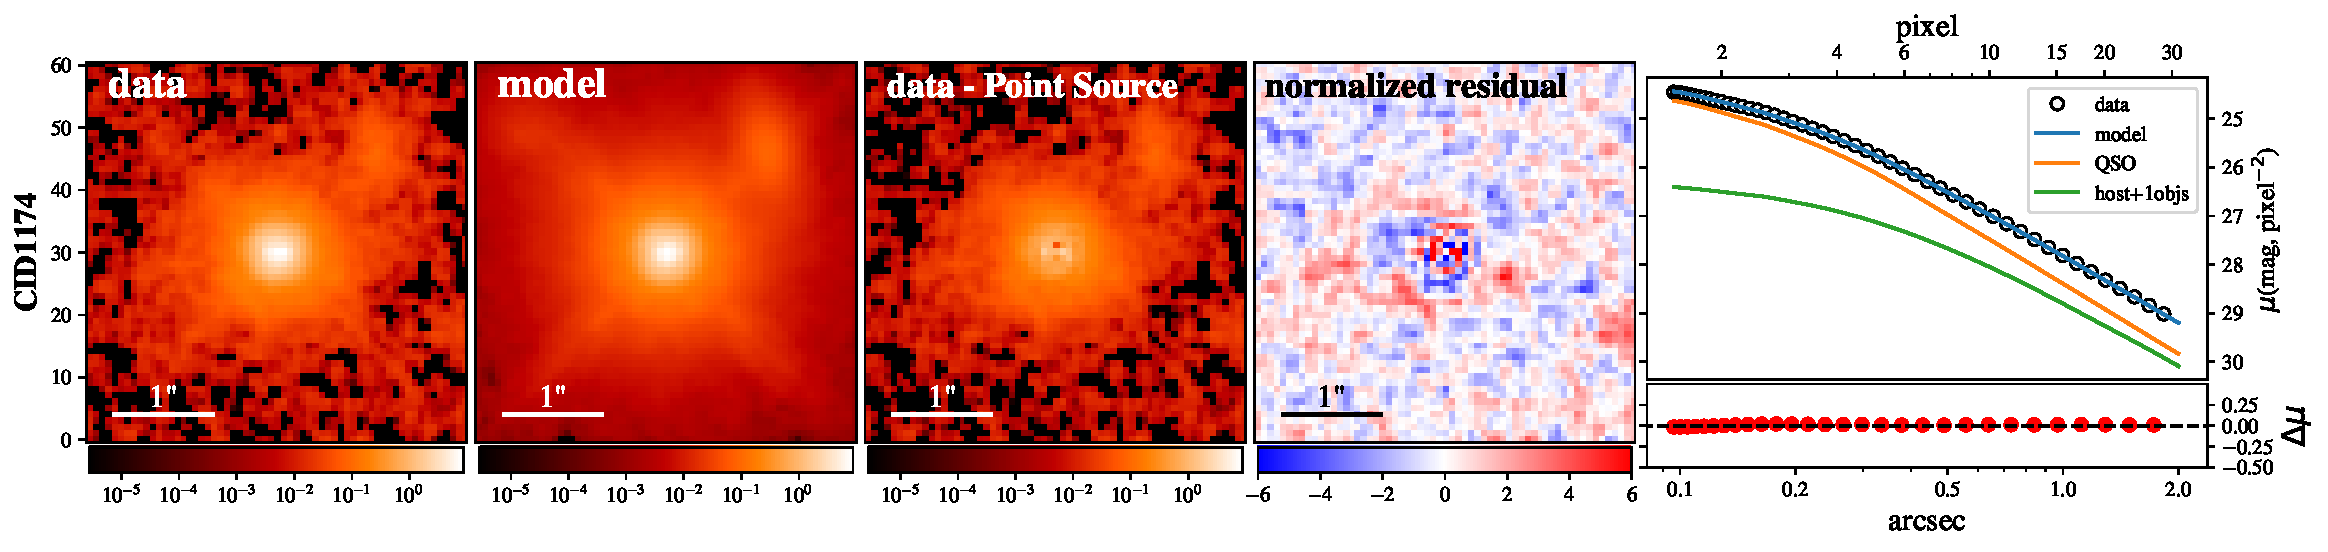
\includegraphics[height=0.25\textwidth]{fig/best_fit_CID1174_SB_profile.pdf}
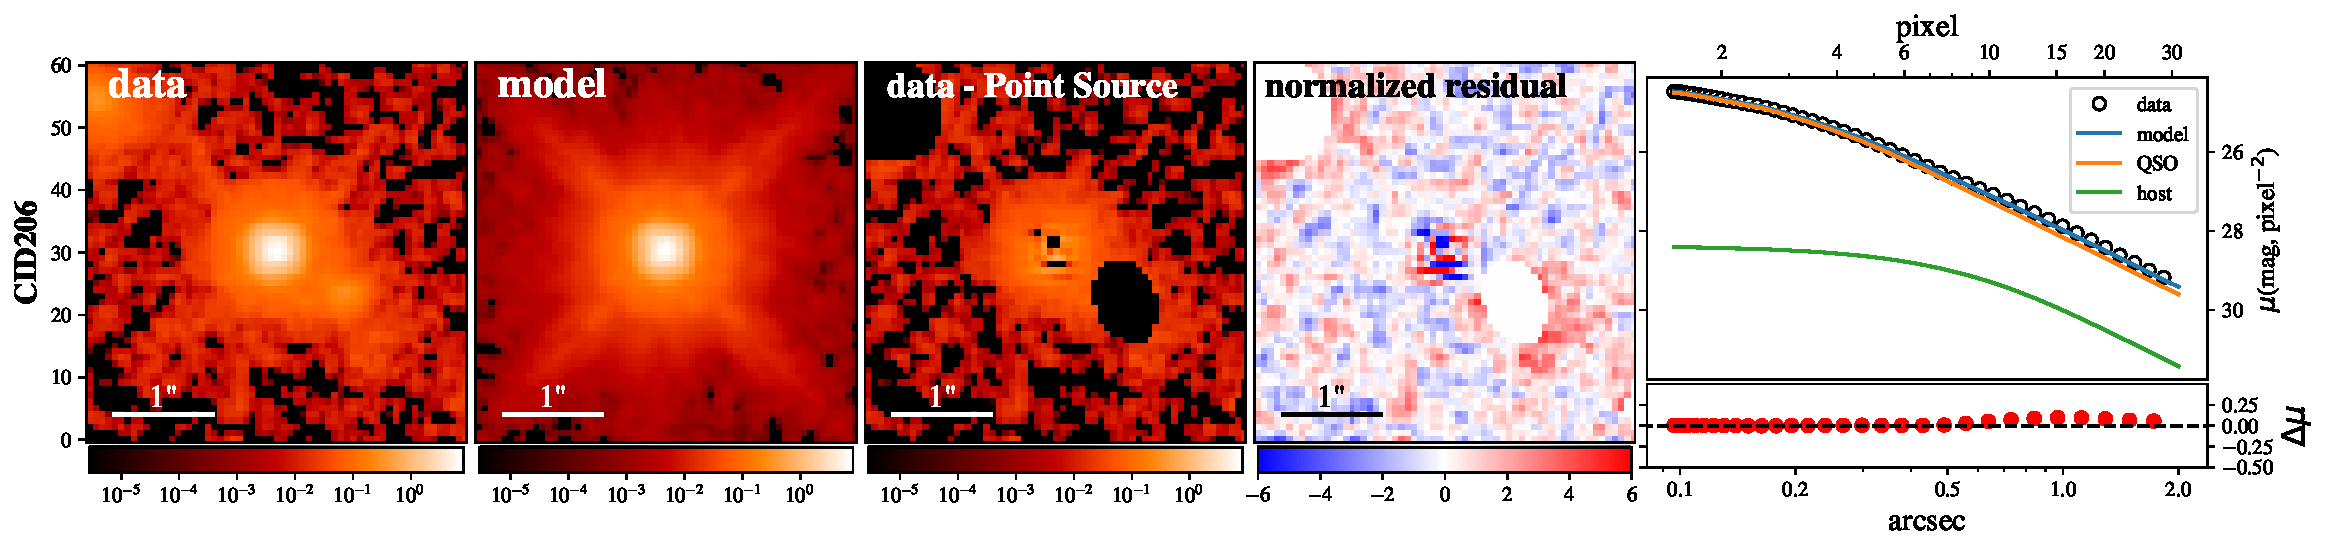
\includegraphics[height=0.25\textwidth]{fig/best_fit_CID206_SB_profile.pdf}
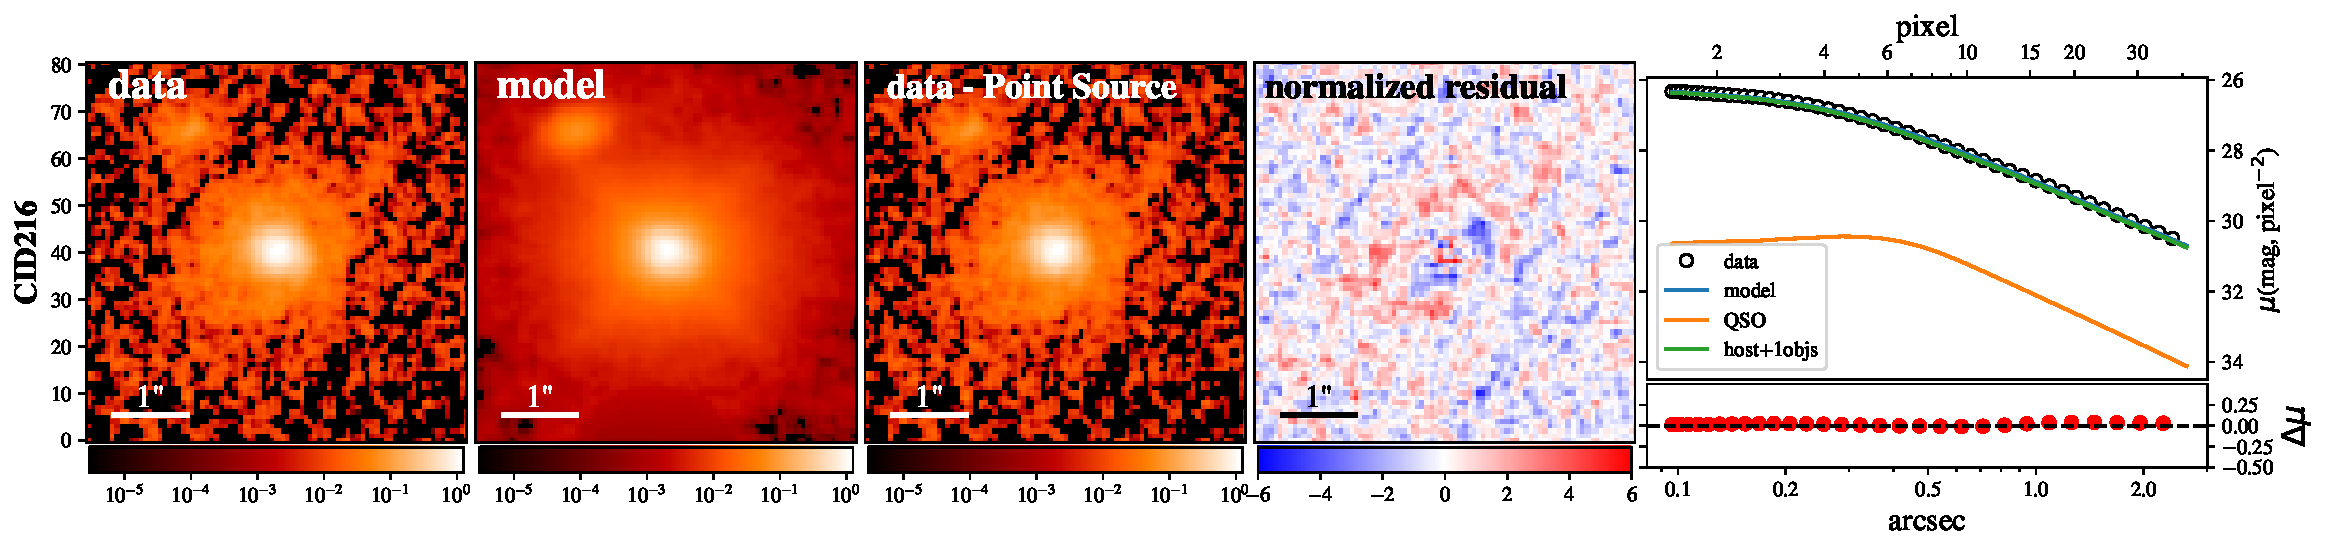
\includegraphics[height=0.25\textwidth]{fig/best_fit_CID216_SB_profile.pdf}
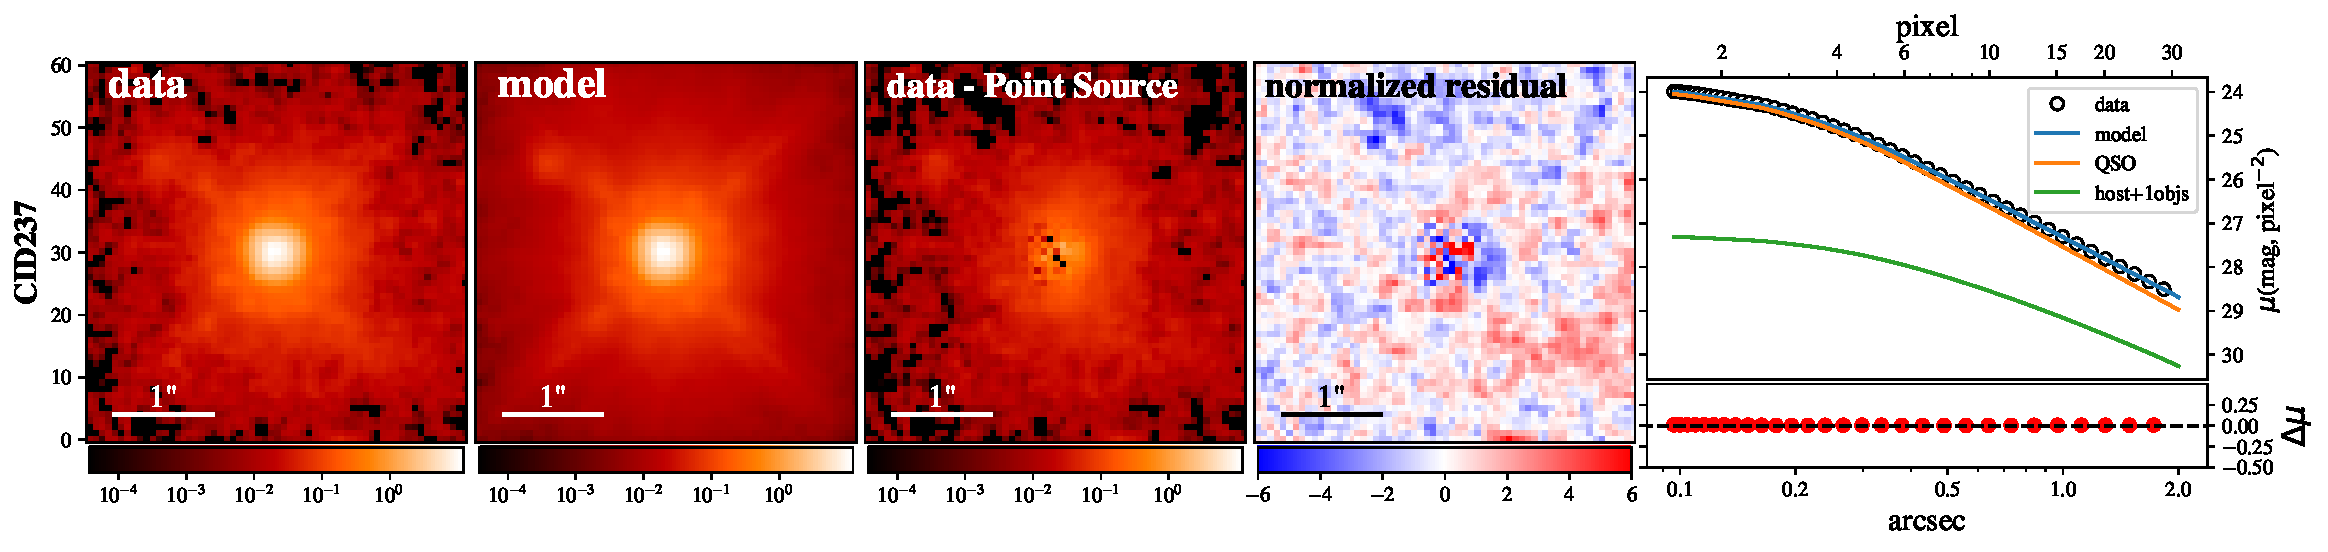
\includegraphics[height=0.25\textwidth]{fig/best_fit_CID237_SB_profile.pdf}
\caption{\label{fig:QSO_decomp} 
\textcolor{red}{need to be written:}
Figure illustrates the inference by WFC3 images for the 34 objects.
In each row, observed data (first column), best-fit models (second column), data subtracted by the inferred point source (third column),  normalized residuals (fourth column) are presented together with the target ID. In the fifth column, we present the 1-D surface brightness profiles and the corresponding residual. \textcolor{blue}{The different colors means blash blash...}
%In each row, observed data (first column), best-fit models (second column), and residuals (third column) are presented with the object name. All images are $10.8\arcsec\times10.8\arcsec$ in size and  displayed with an inverted asinh stretch. The fourth column shows the corresponding one-dimensional surface brightness profiles. In each top panel, the profiles measured from the data (open circles), the best-fit model (black solid line), and the sub-components of the model for bulge (blue solid line), disk (green solid line), AGN (red solid line) are shown. Residuals (gray circles), the difference of the profiles between the data and the best-fit model, are presented in each bottom panel. Note that the one-dimensional surface brightness profiles are shown for illustration purposes only, the actual fitting made use of the full two-dimensional images.
}}
\end{figure*} 

\begin{figure*}
\centering
%\hspace{-5.5em}
{
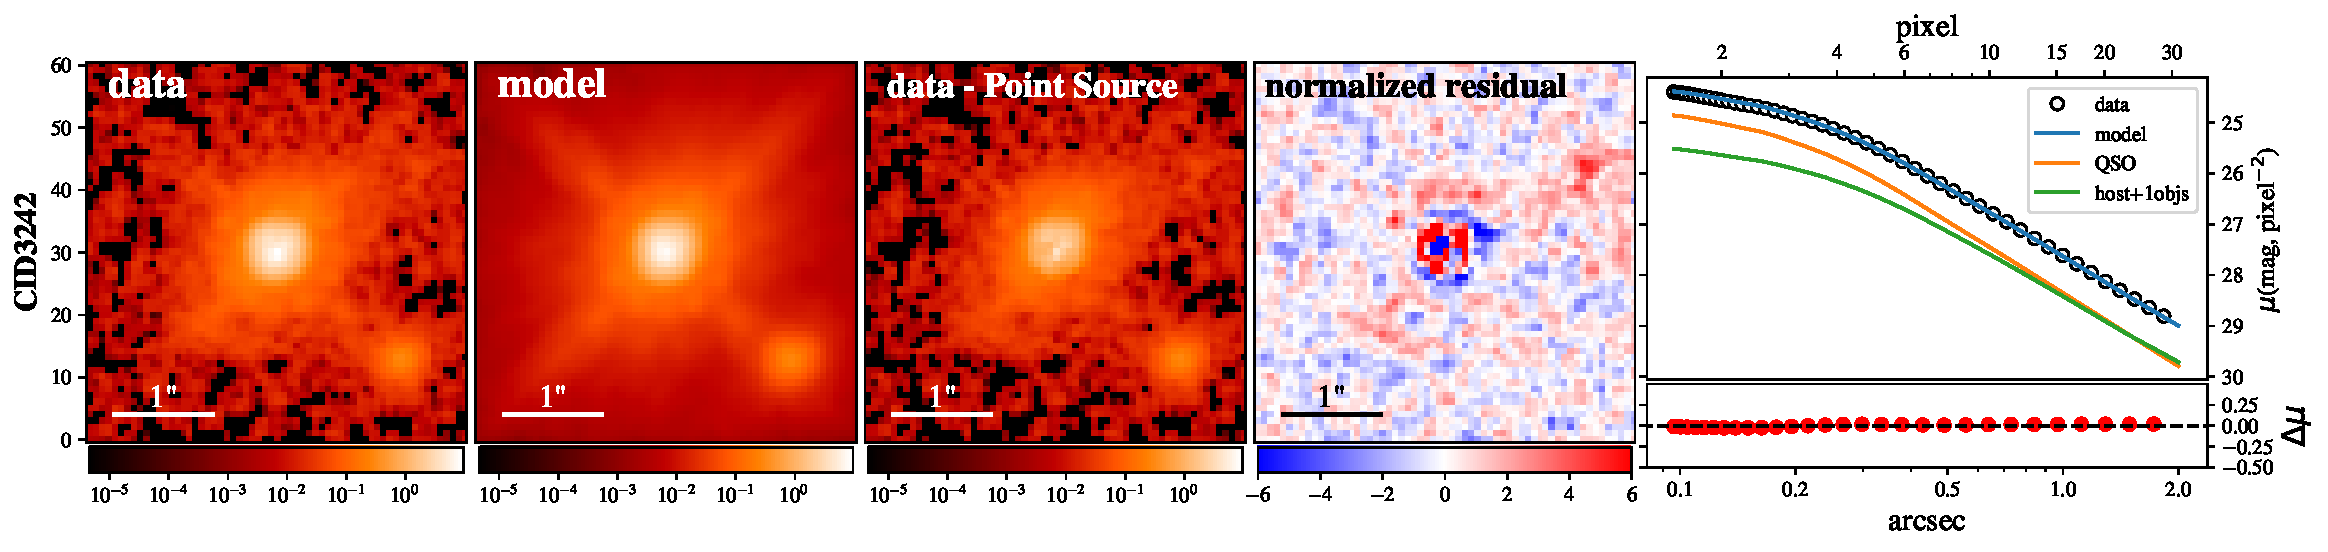
\includegraphics[height=0.25\textwidth]{fig/best_fit_CID3242_SB_profile.pdf}
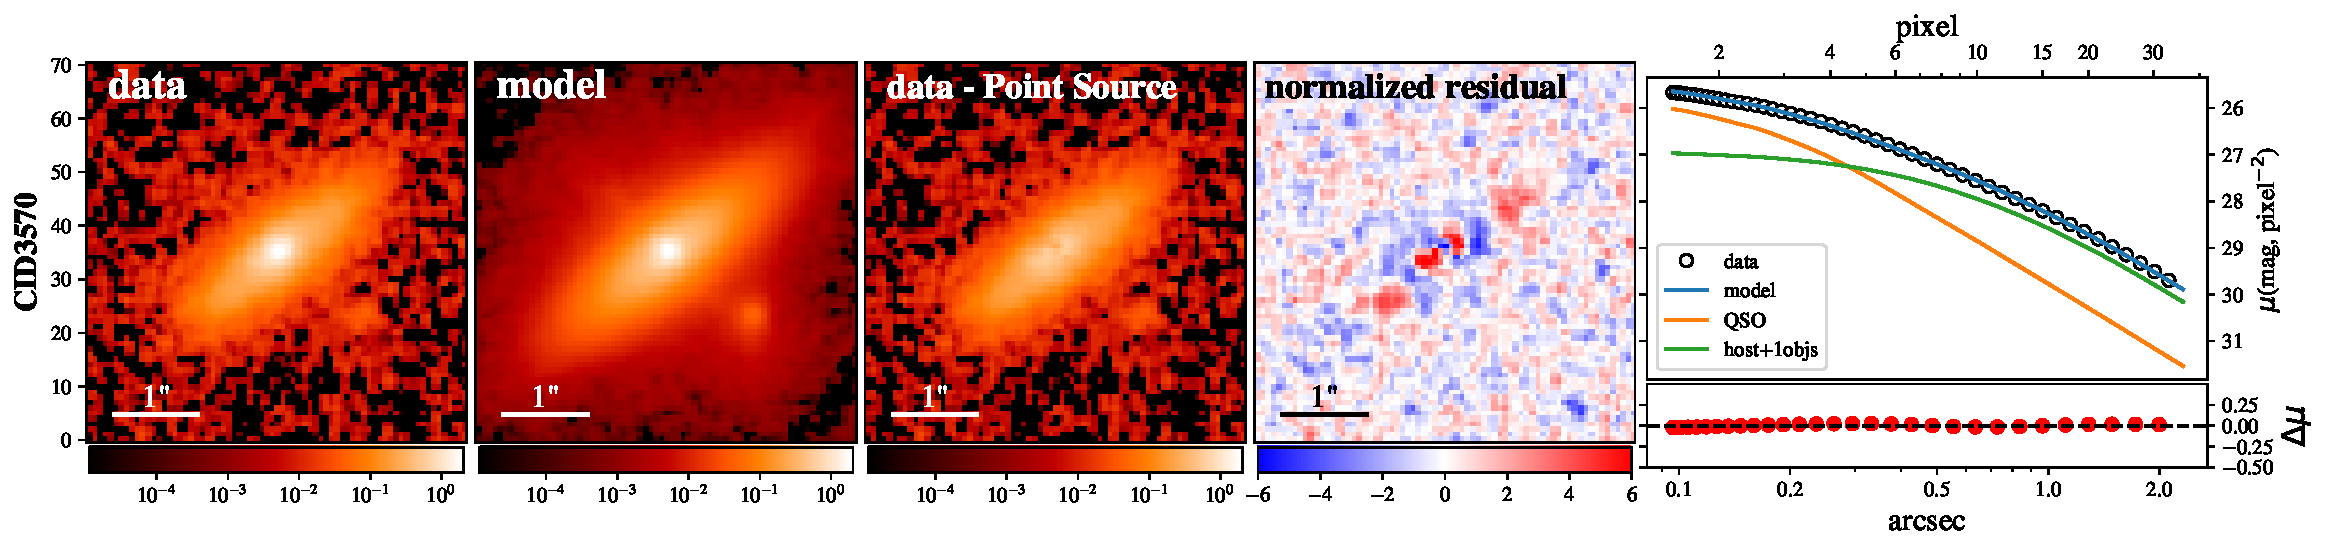
\includegraphics[height=0.25\textwidth]{fig/best_fit_CID3570_SB_profile.pdf}
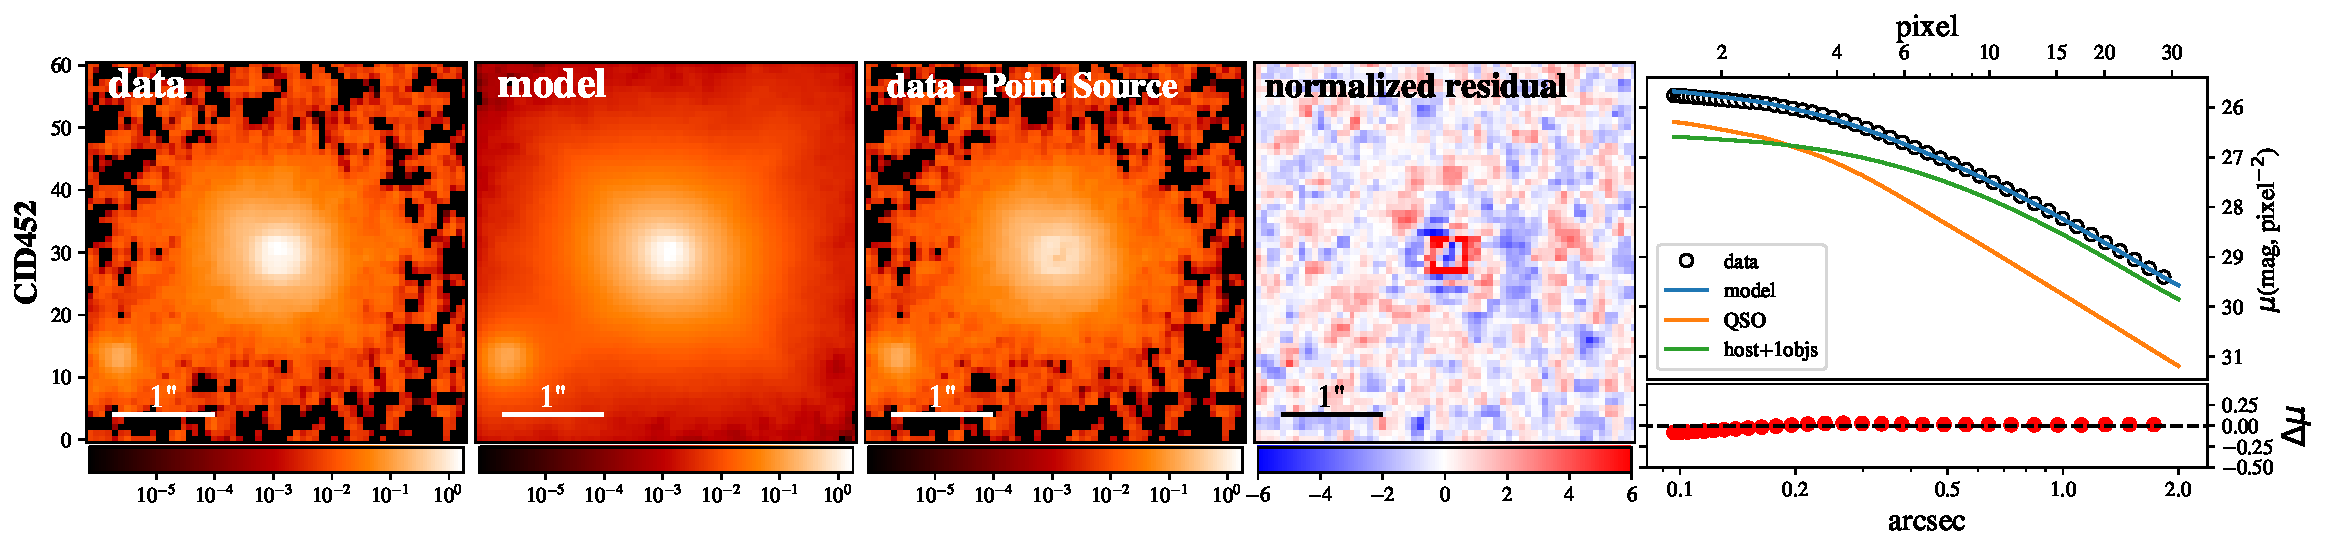
\includegraphics[height=0.25\textwidth]{fig/best_fit_CID452_SB_profile.pdf}
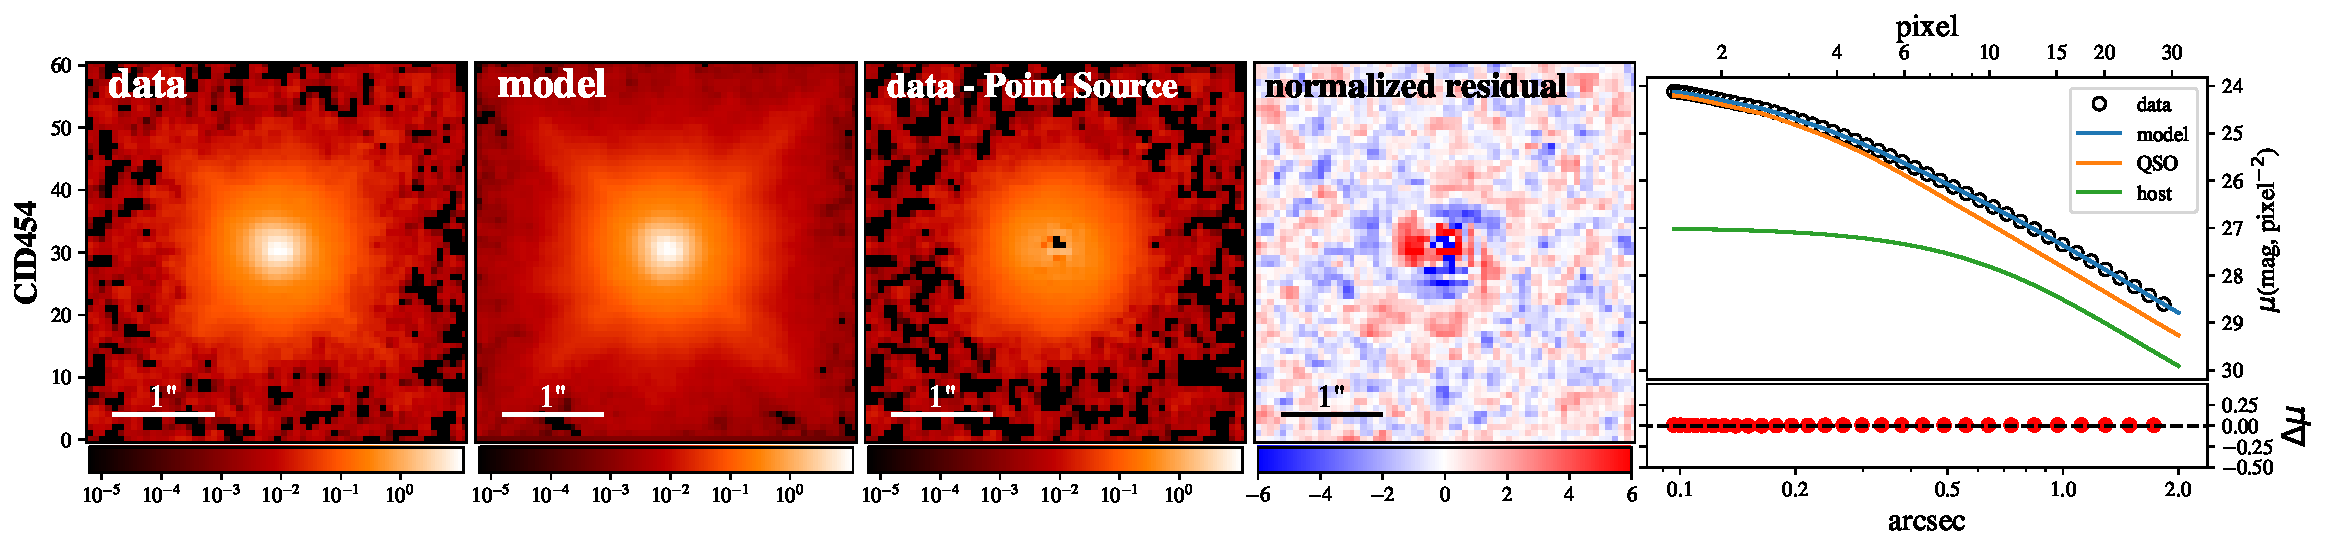
\includegraphics[height=0.25\textwidth]{fig/best_fit_CID454_SB_profile.pdf}
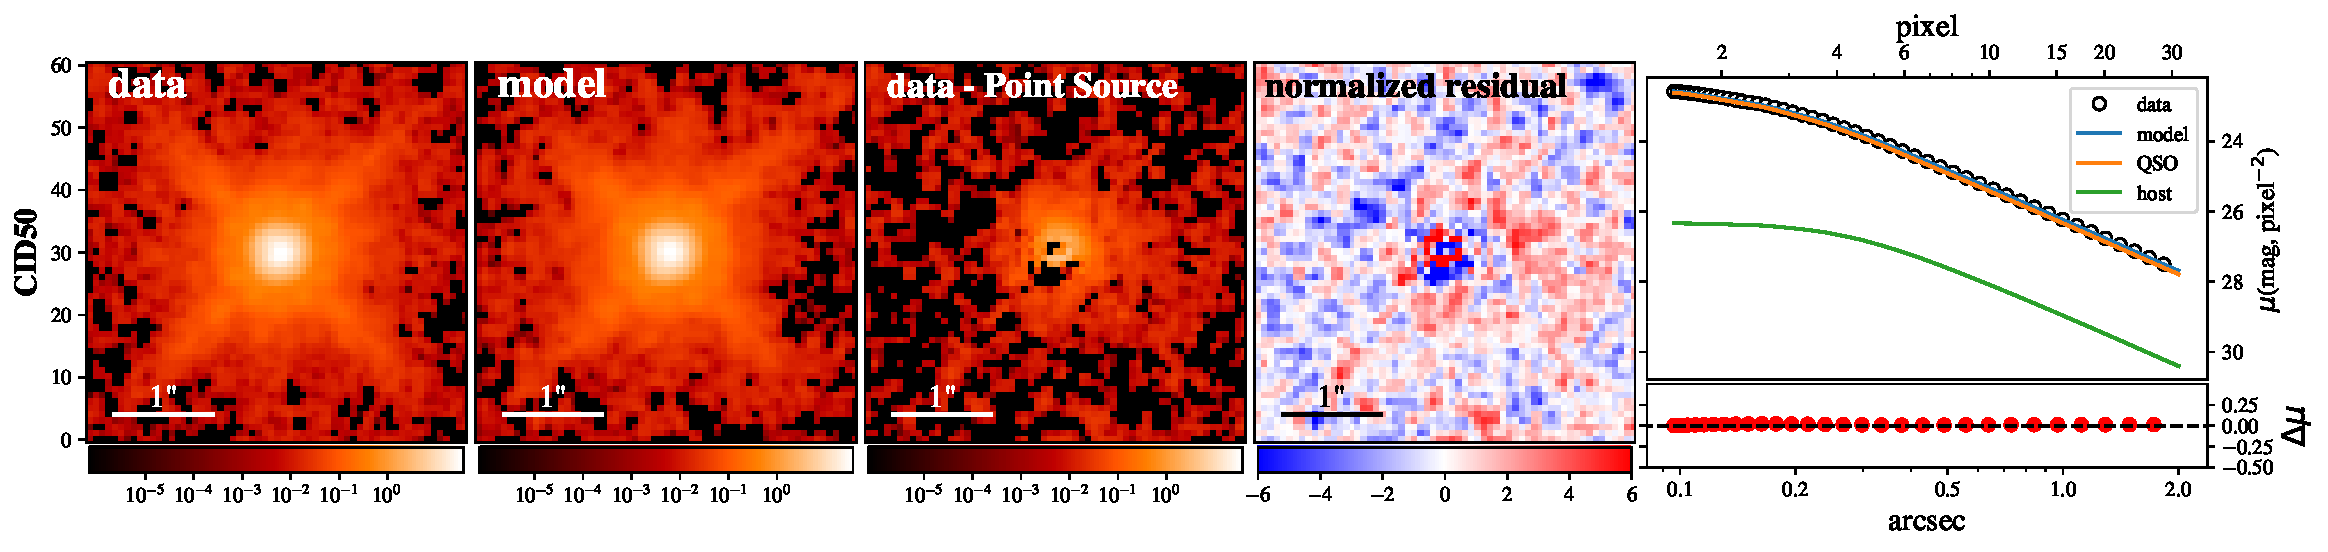
\includegraphics[height=0.25\textwidth]{fig/best_fit_CID50_SB_profile.pdf}
}
\figurenum{1}
\caption{Continued.}
\end{figure*} 

\begin{figure*}
\centering
%\hspace{-5.5em}
{
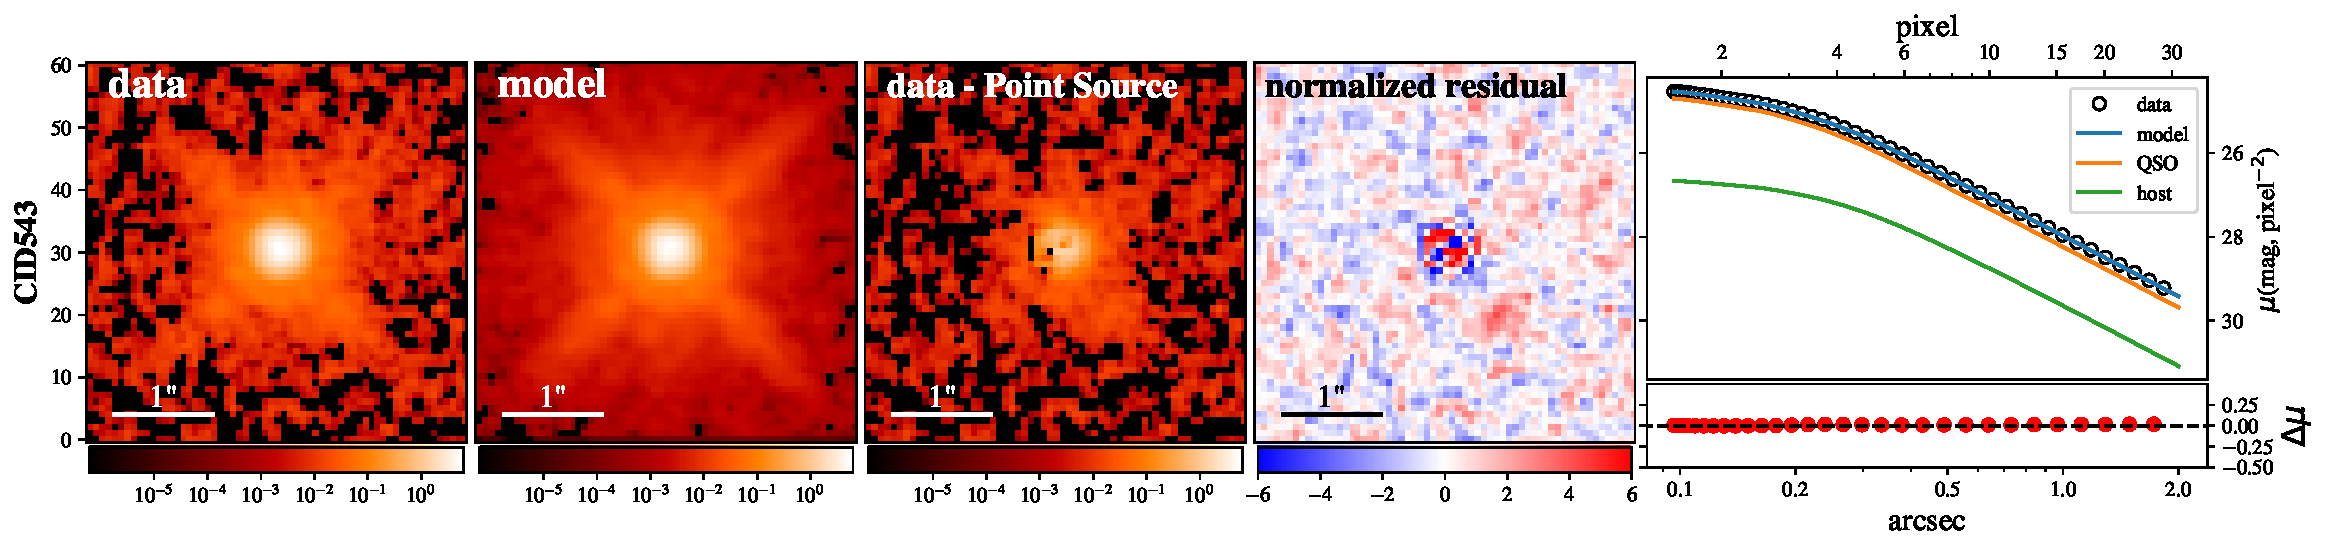
\includegraphics[height=0.25\textwidth]{fig/best_fit_CID543_SB_profile.pdf}
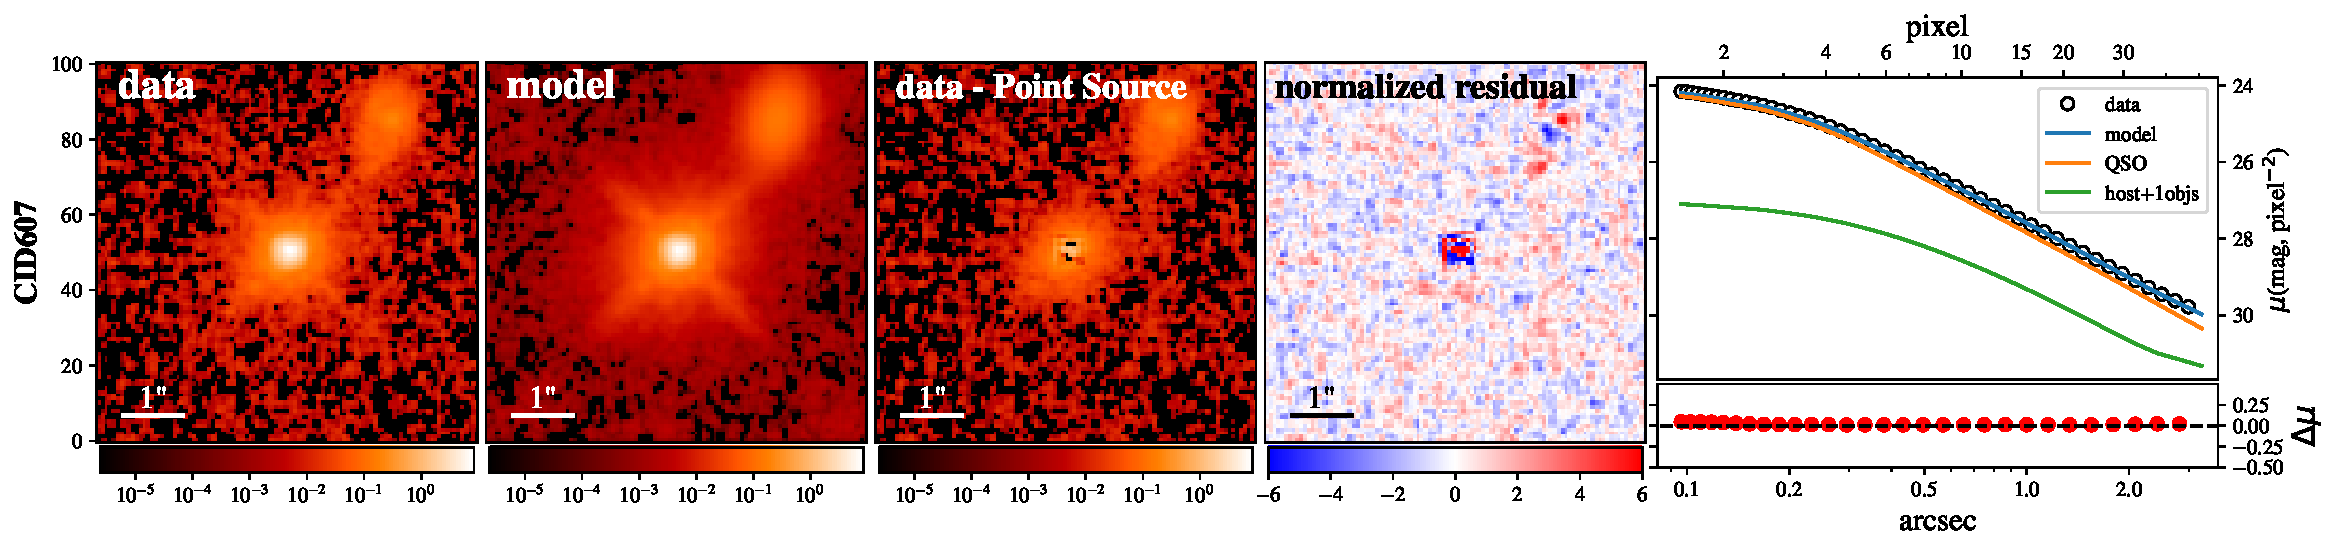
\includegraphics[height=0.25\textwidth]{fig/best_fit_CID607_SB_profile.pdf}
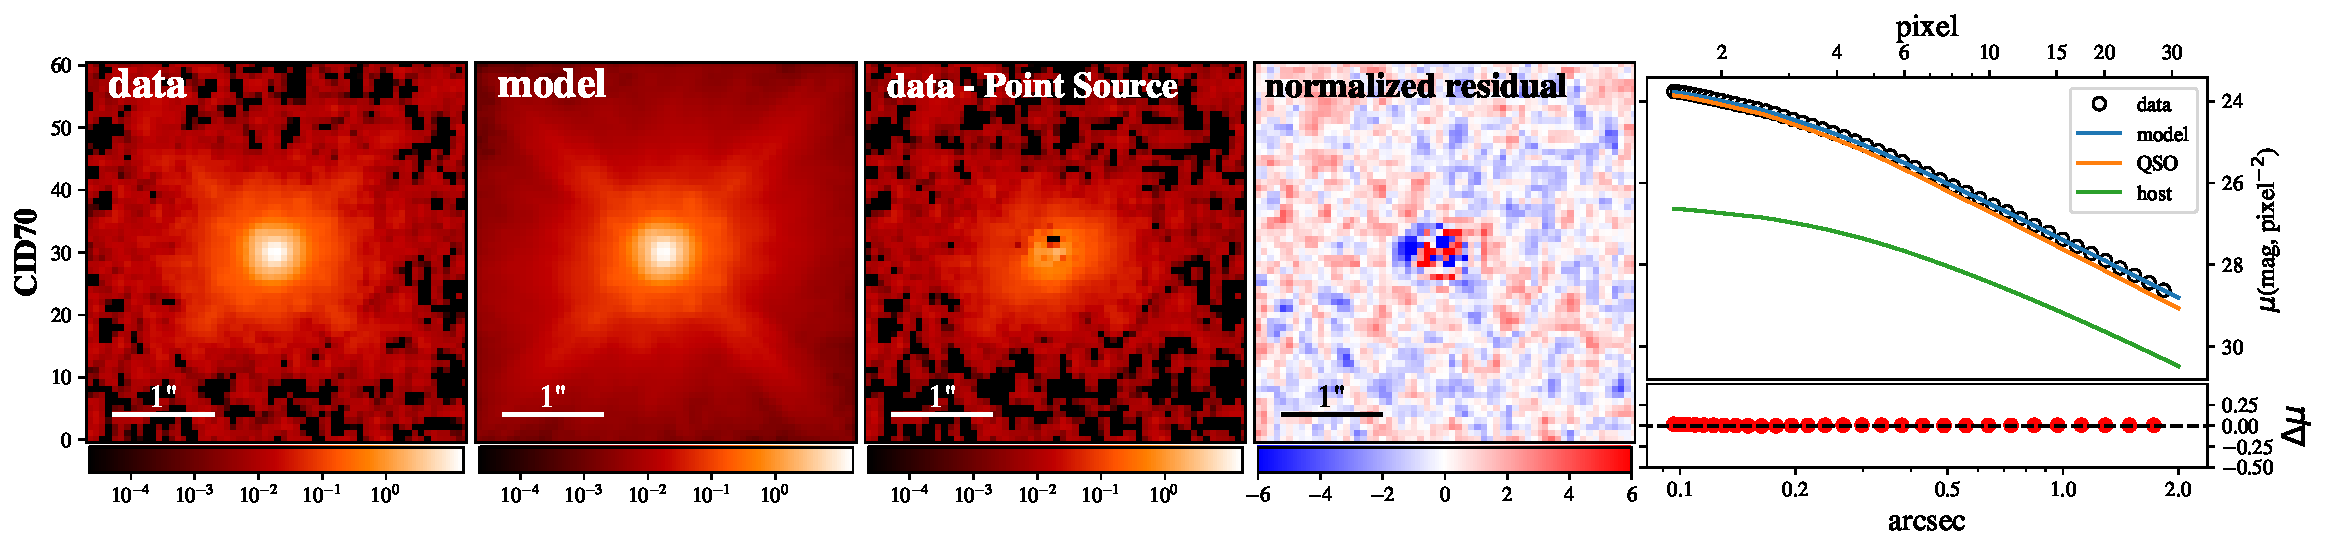
\includegraphics[height=0.25\textwidth]{fig/best_fit_CID70_SB_profile.pdf}
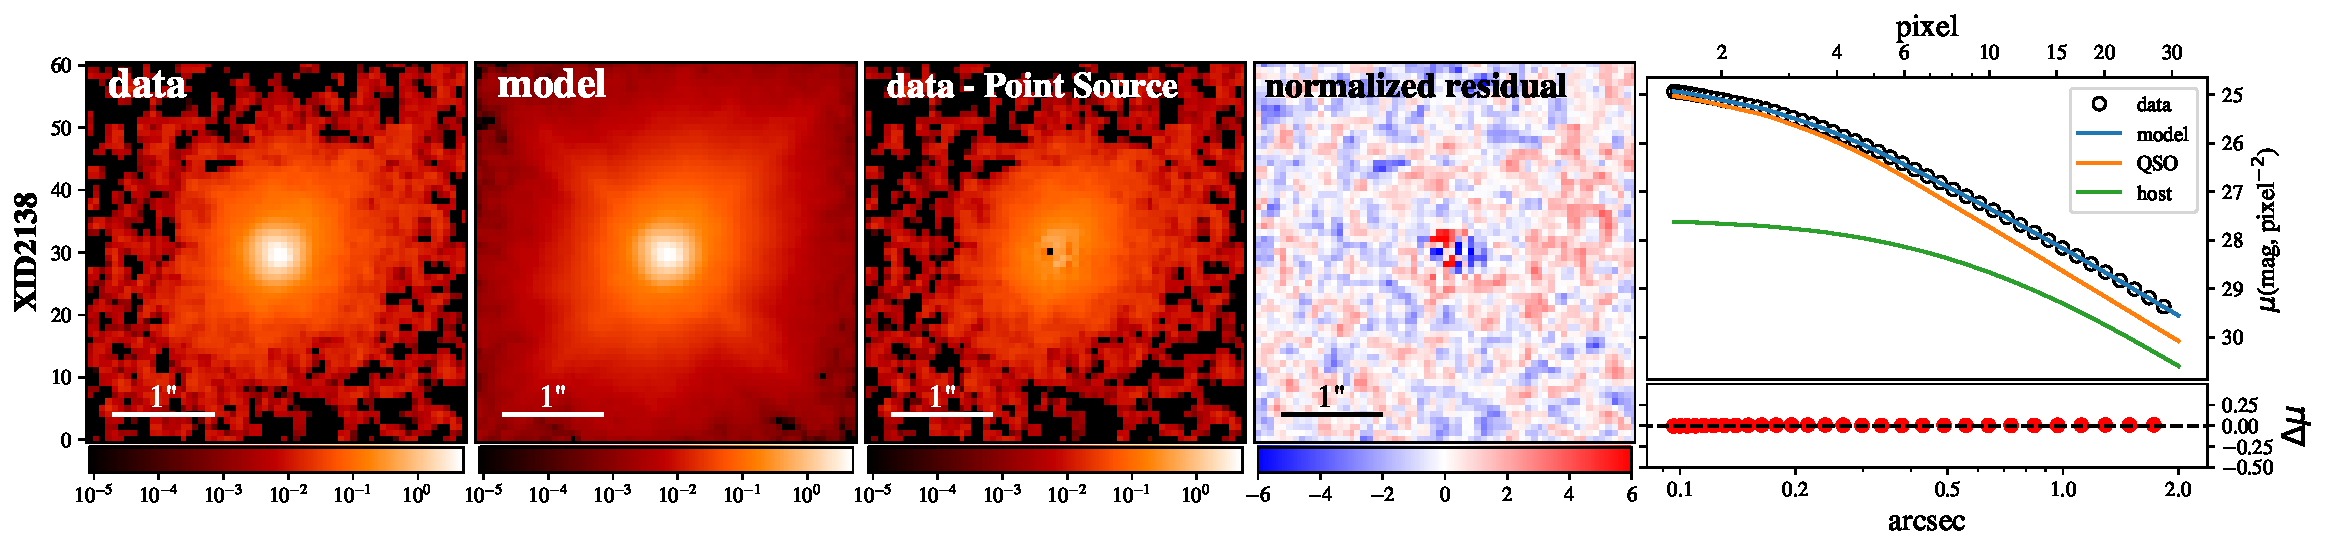
\includegraphics[height=0.25\textwidth]{fig/best_fit_XID2138_SB_profile.pdf}
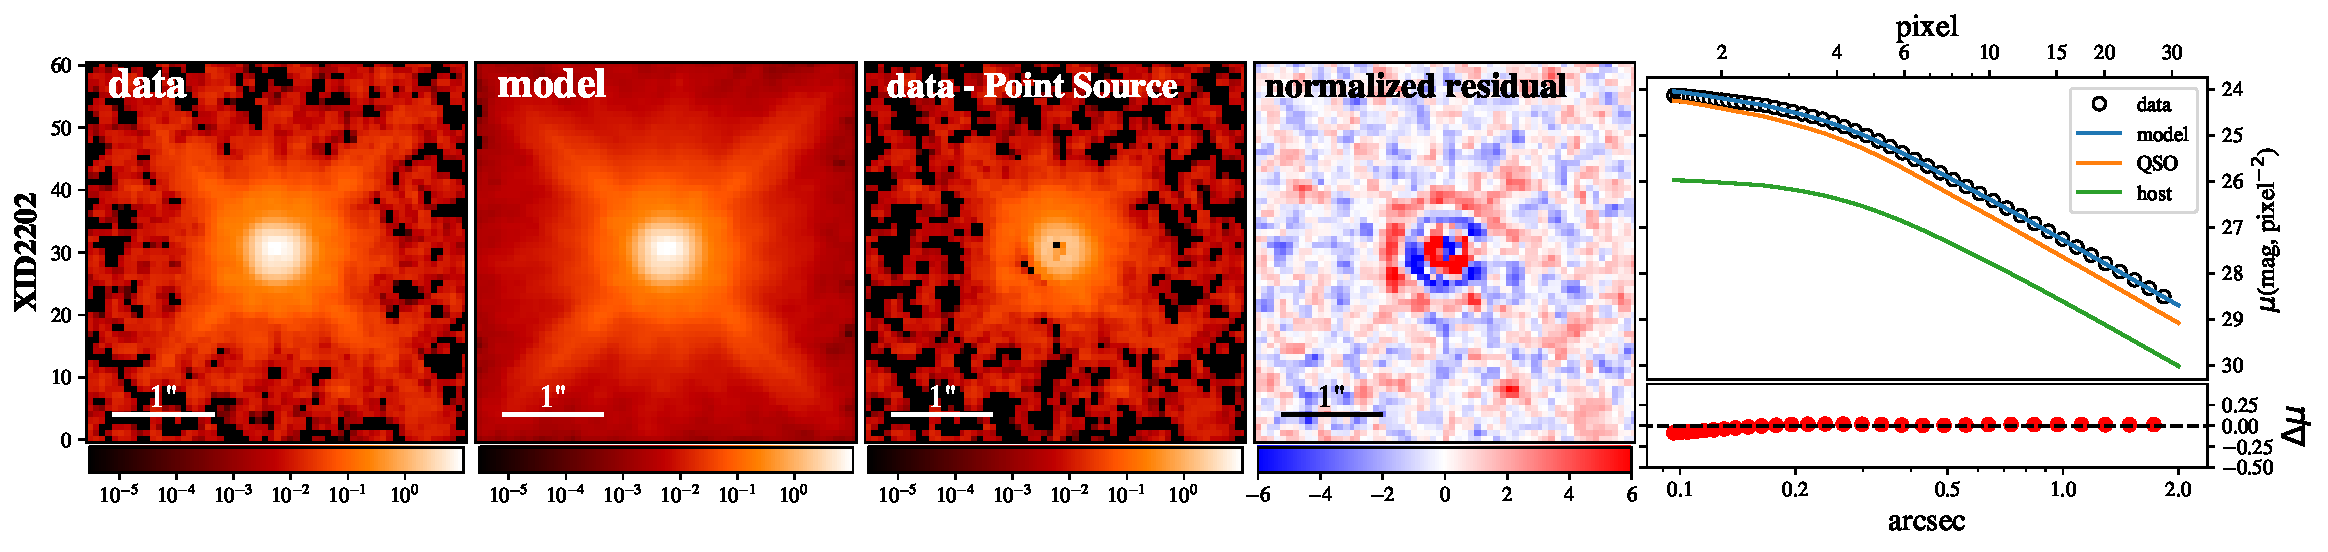
\includegraphics[height=0.25\textwidth]{fig/best_fit_XID2202_SB_profile.pdf}
}
\figurenum{1}
\caption{Continued.}
\end{figure*} 

\begin{figure*}
\centering
%\hspace{-5.5em}
{
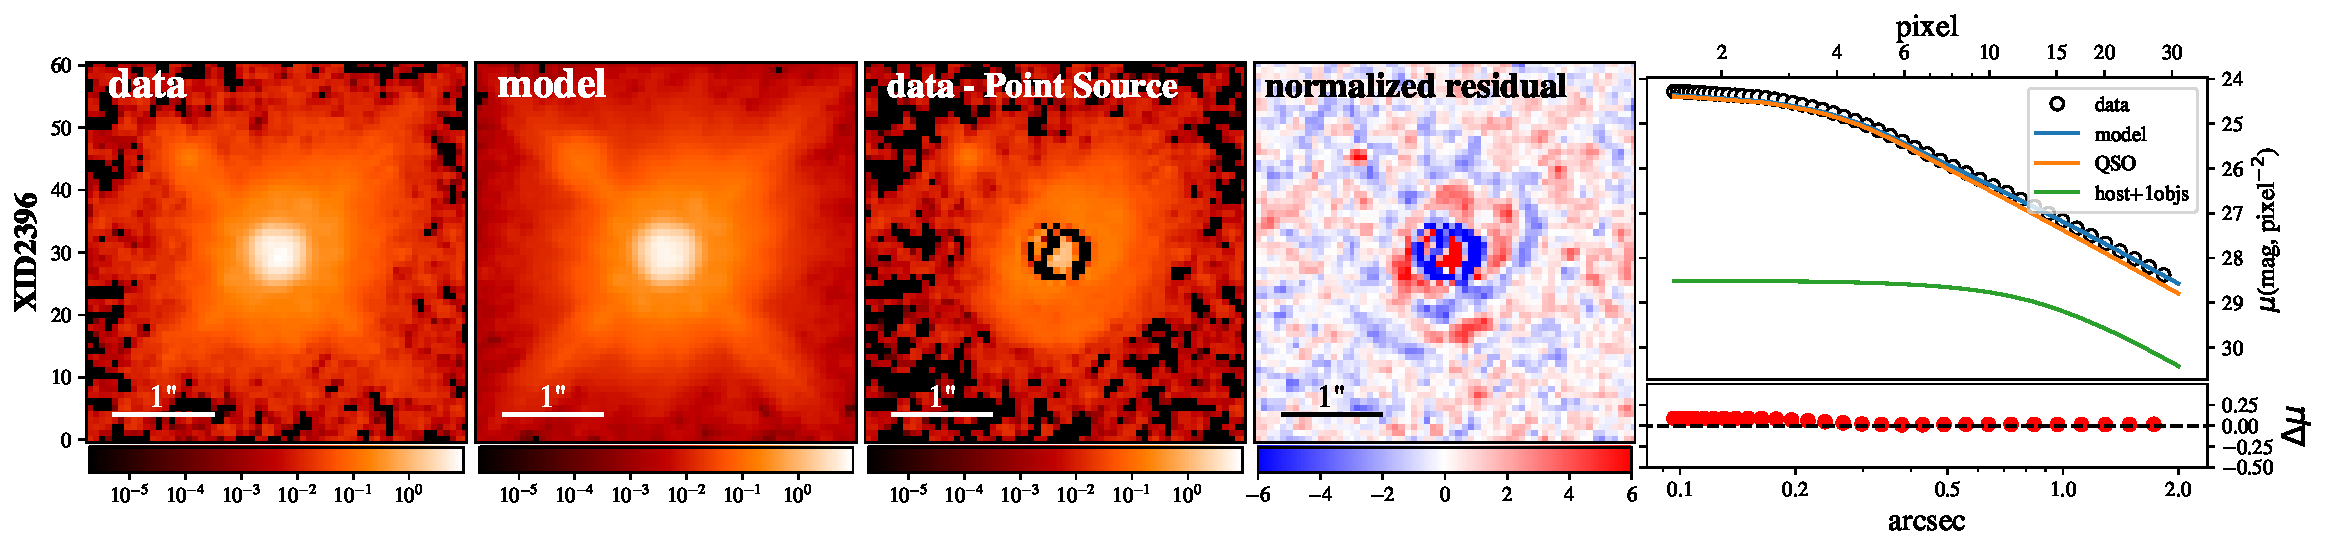
\includegraphics[height=0.25\textwidth]{fig/best_fit_XID2396_SB_profile.pdf}
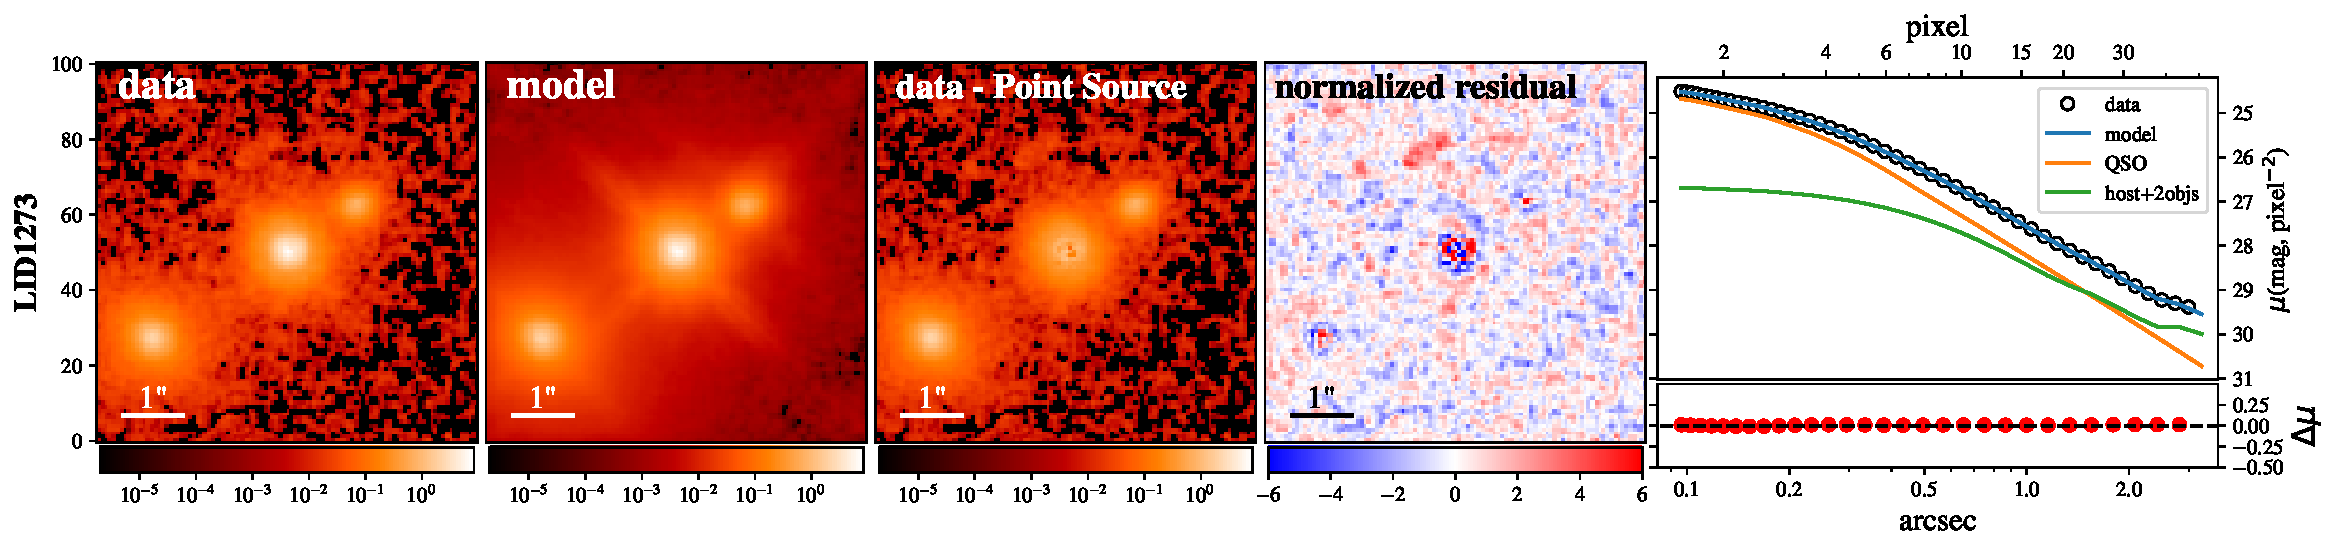
\includegraphics[height=0.25\textwidth]{fig/best_fit_LID1273_SB_profile.pdf}
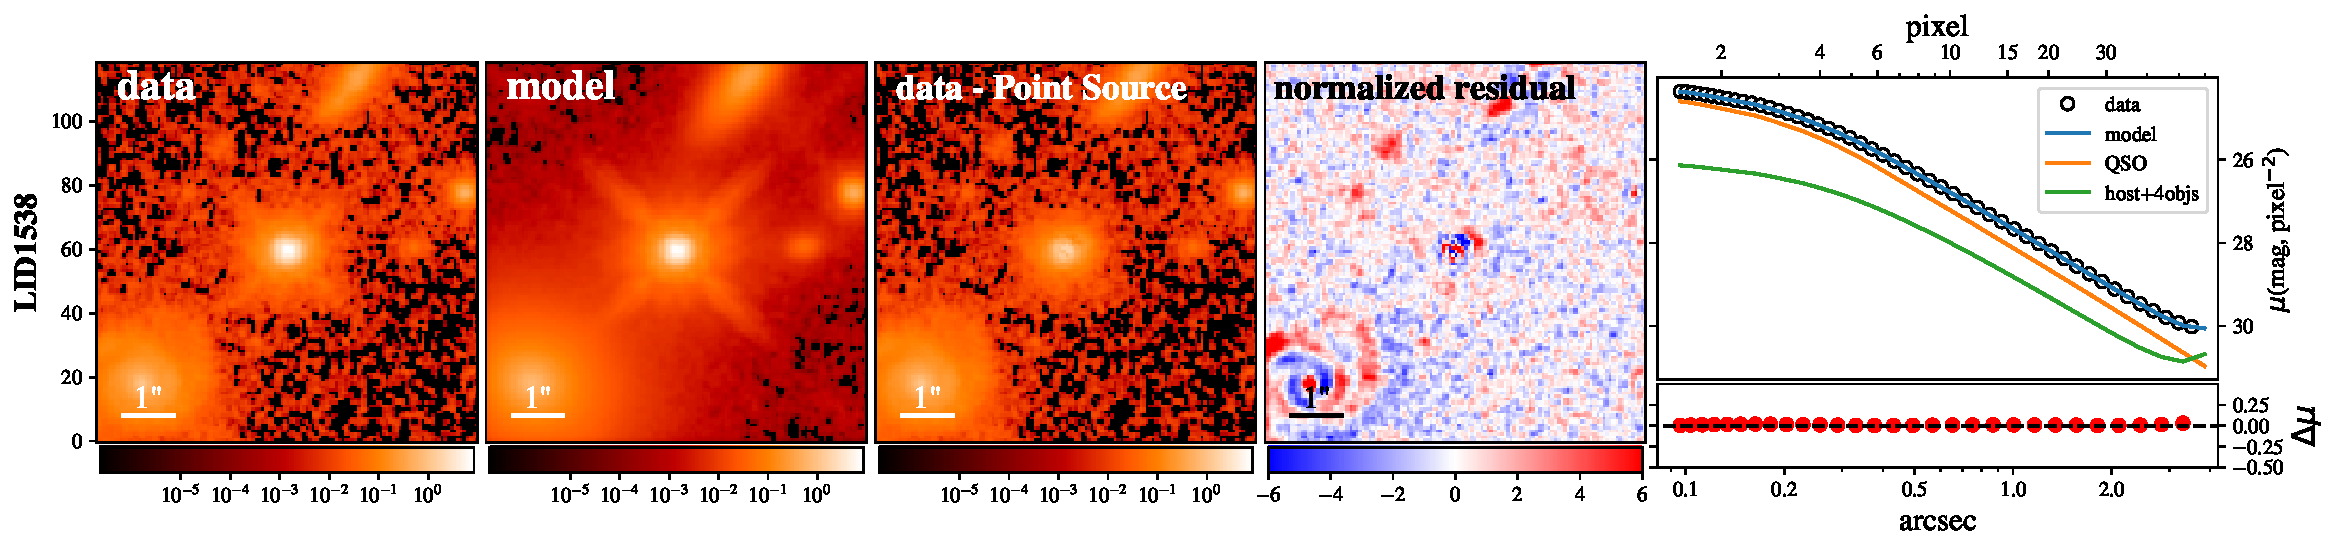
\includegraphics[height=0.25\textwidth]{fig/best_fit_LID1538_SB_profile.pdf}
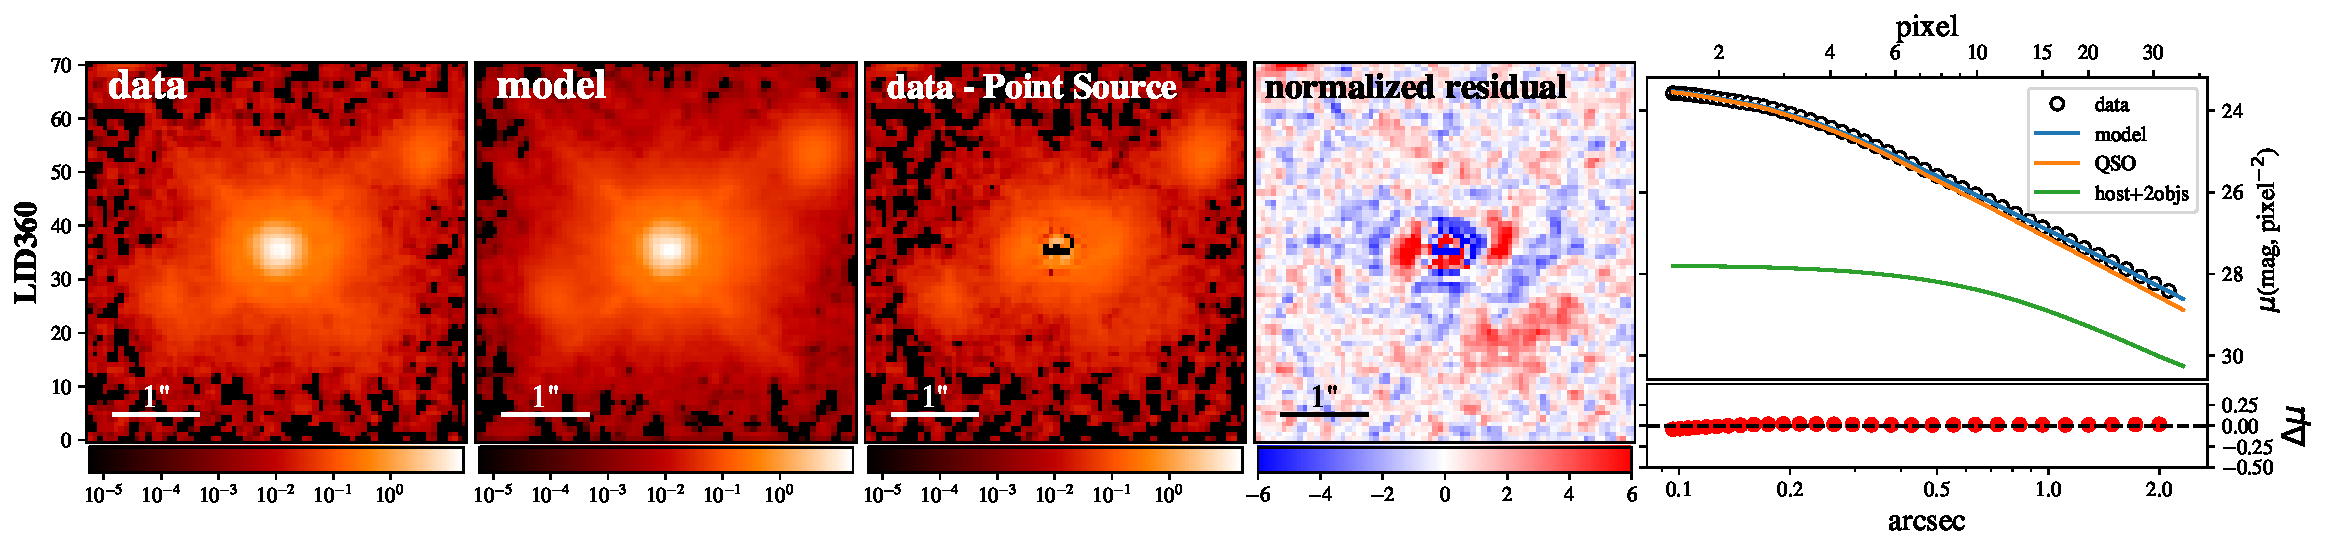
\includegraphics[height=0.25\textwidth]{fig/best_fit_LID360_SB_profile.pdf}
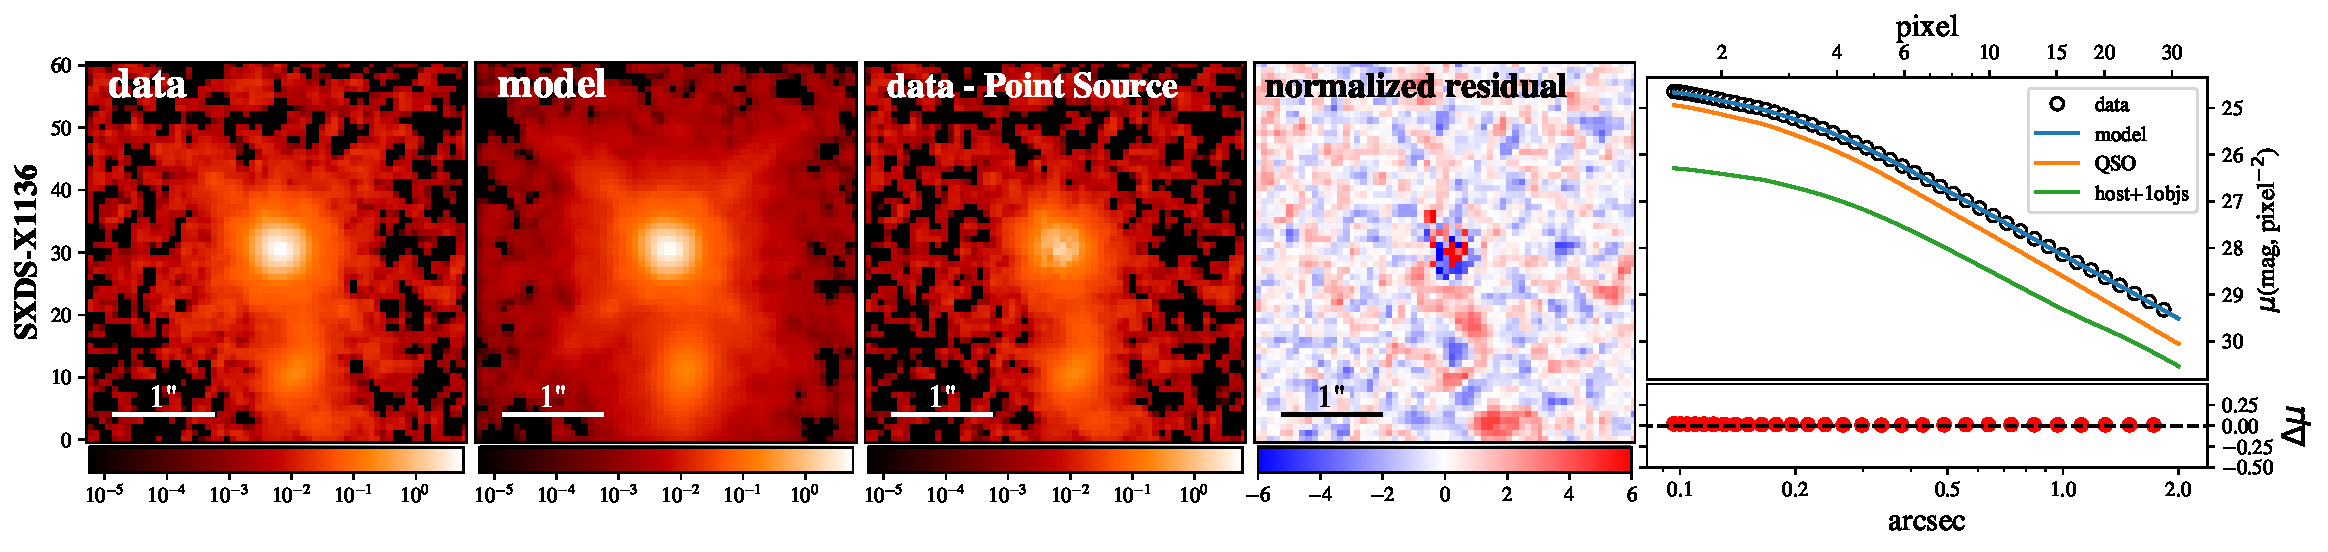
\includegraphics[height=0.25\textwidth]{fig/best_fit_SXDS-X1136_SB_profile.pdf}
}
\figurenum{1}
\caption{Continued.}
\end{figure*} 

\begin{figure*}
\centering
%\hspace{-5.5em}
{
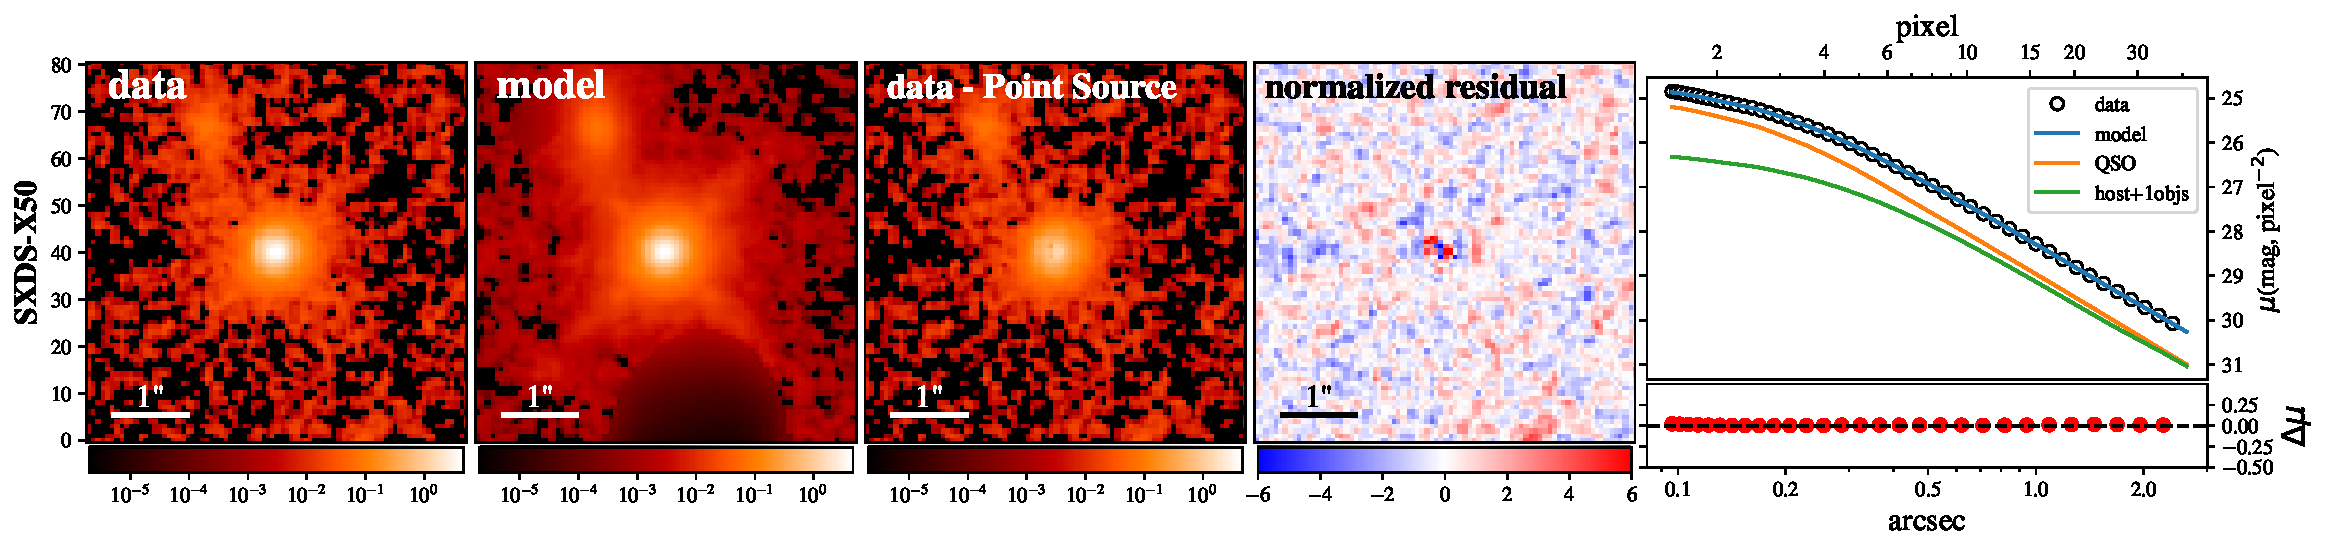
\includegraphics[height=0.25\textwidth]{fig/best_fit_SXDS-X50_SB_profile.pdf}
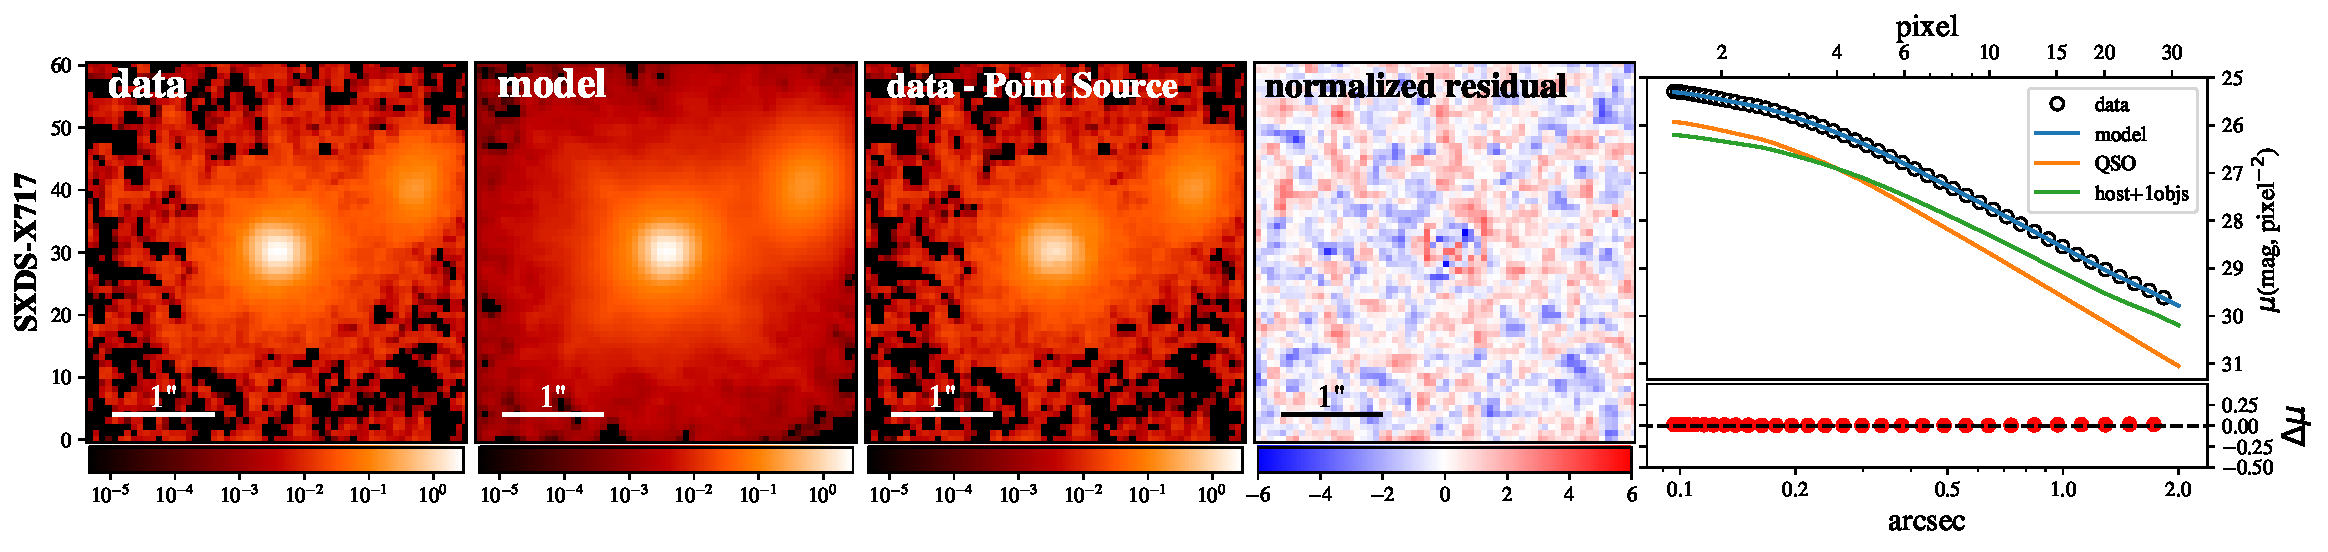
\includegraphics[height=0.25\textwidth]{fig/best_fit_SXDS-X717_SB_profile.pdf}
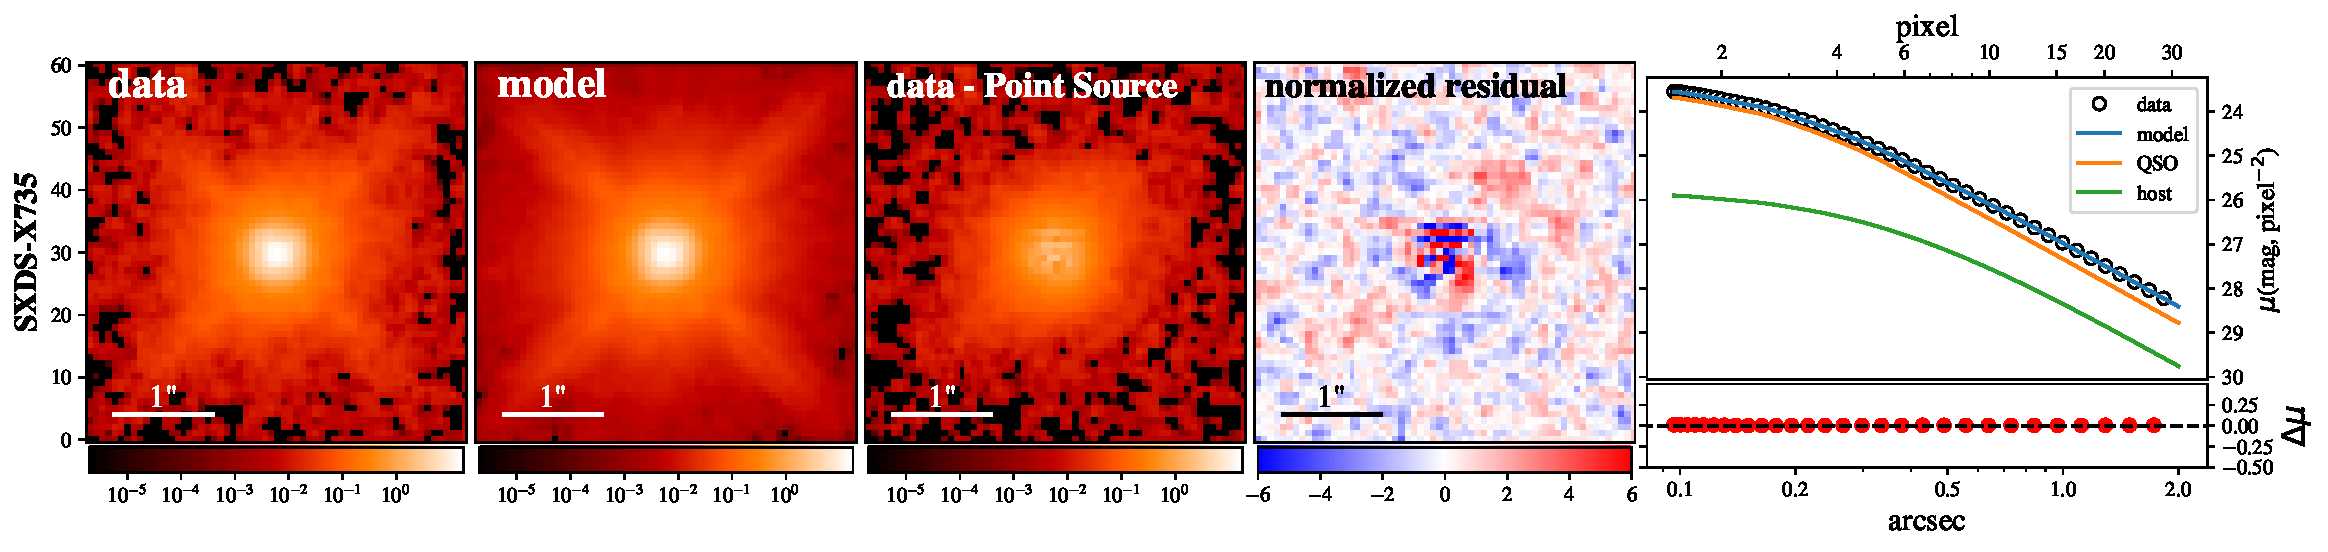
\includegraphics[height=0.25\textwidth]{fig/best_fit_SXDS-X735_SB_profile.pdf}
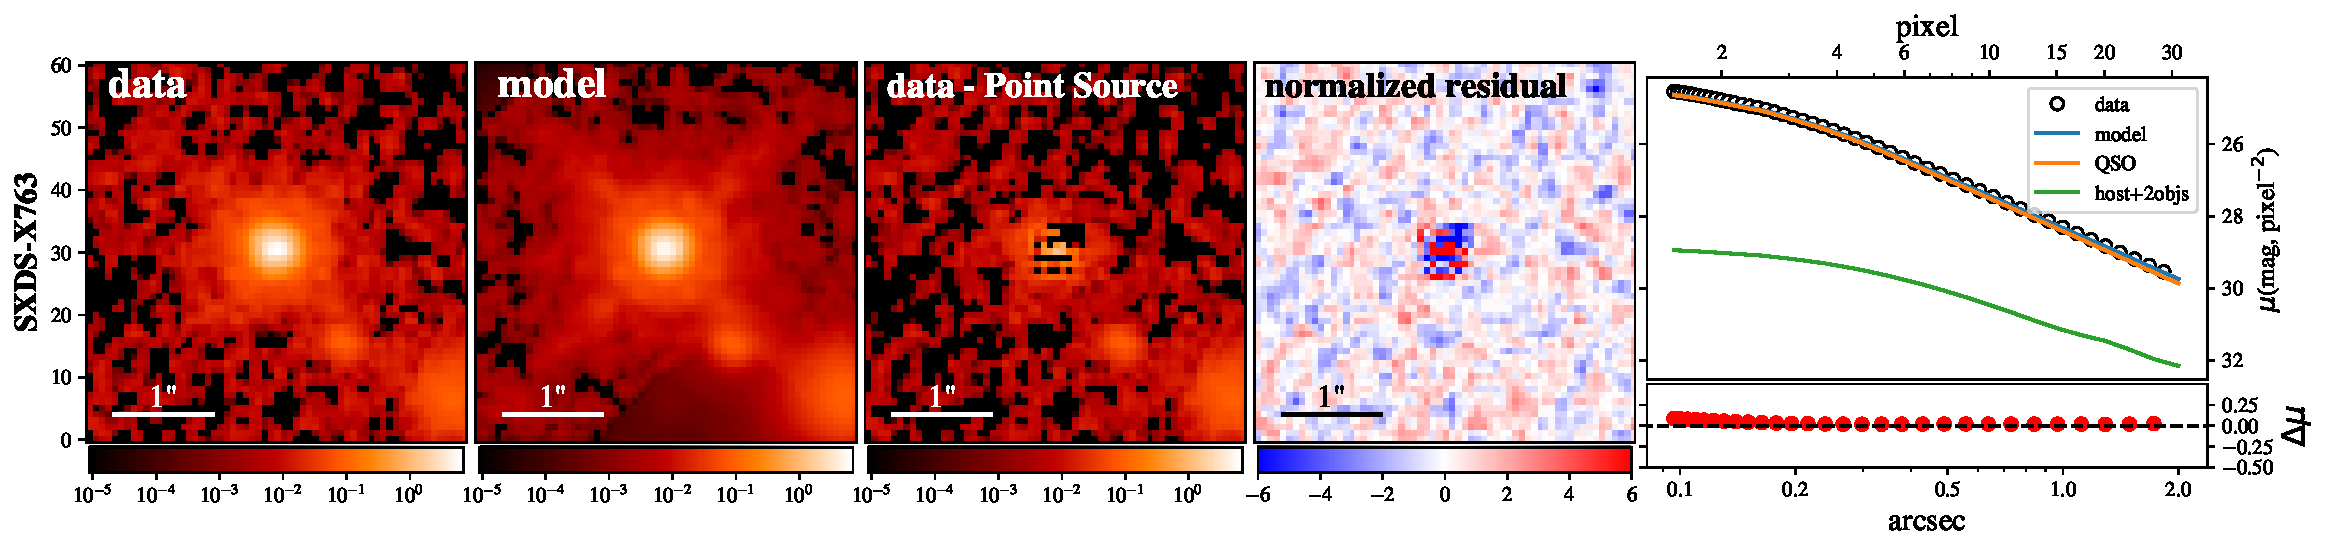
\includegraphics[height=0.25\textwidth]{fig/best_fit_SXDS-X763_SB_profile.pdf}
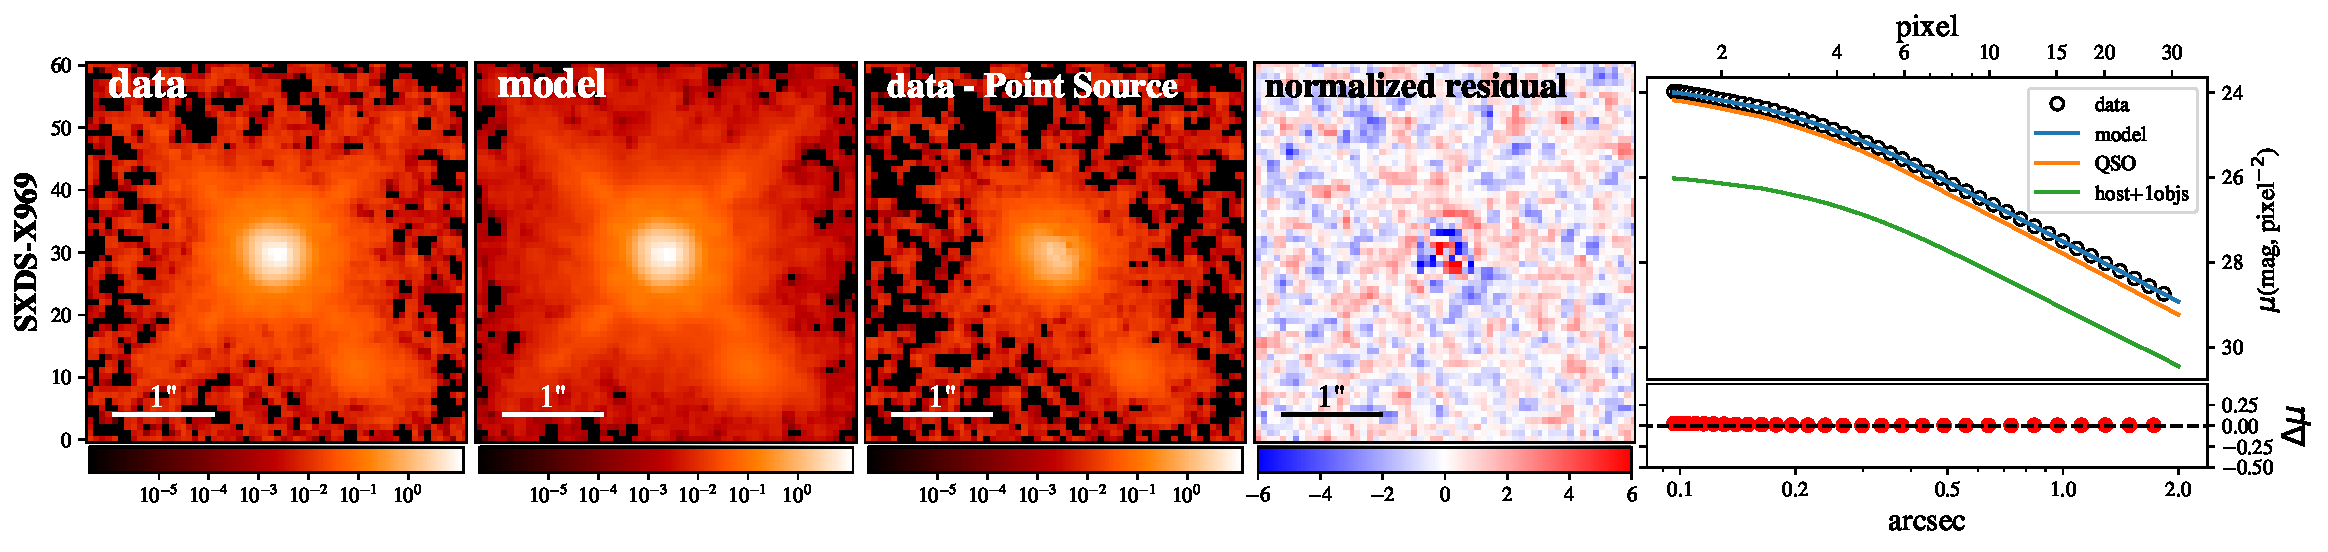
\includegraphics[height=0.25\textwidth]{fig/best_fit_SXDS-X969_SB_profile.pdf}
}
\figurenum{1}
\caption{Continued.}
\end{figure*} 

\begin{figure*}
\centering
%\hspace{-5.5em}
{
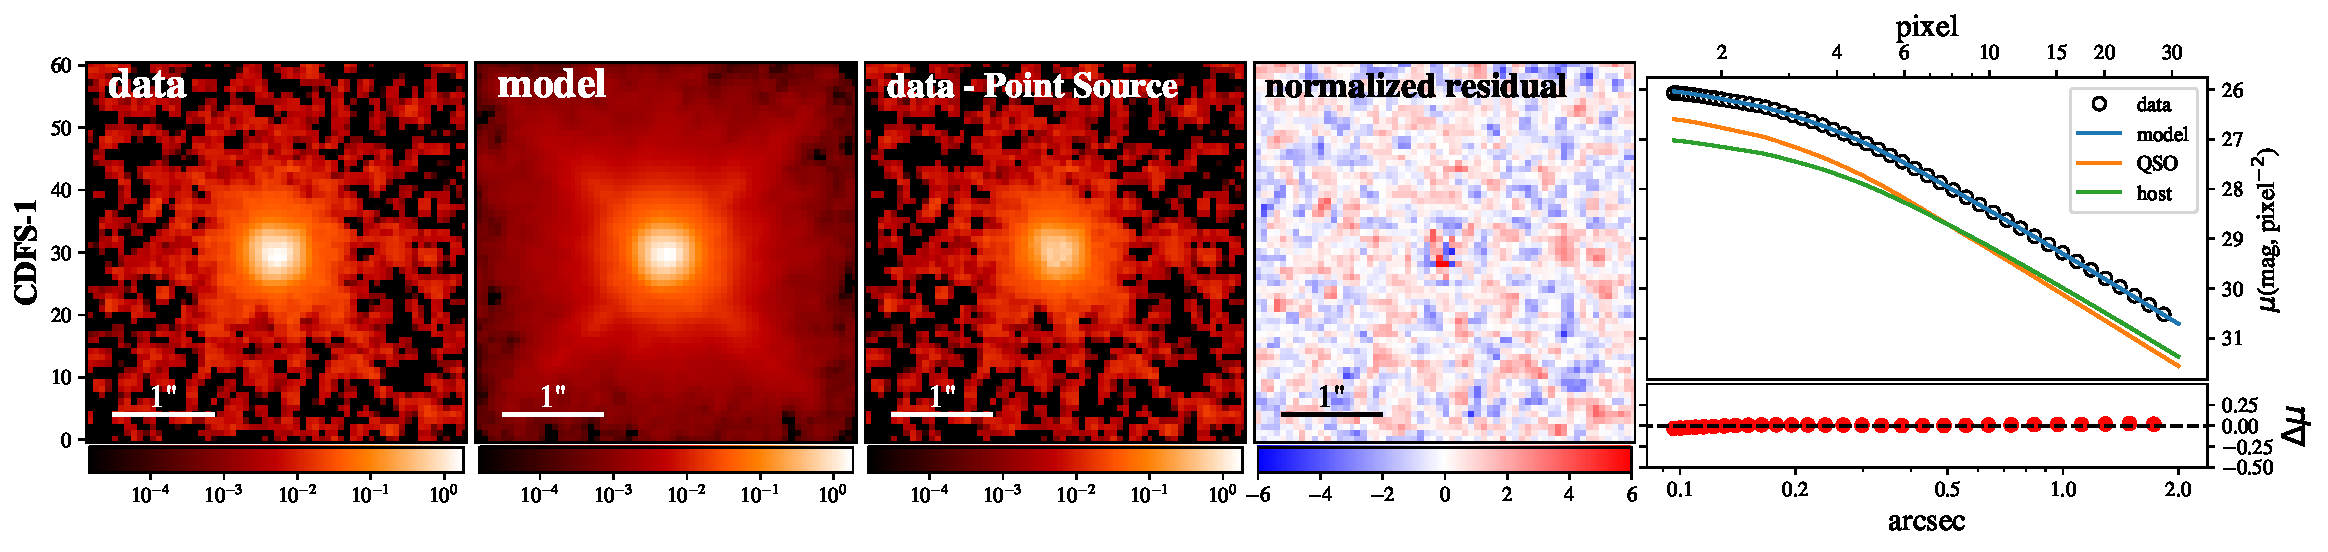
\includegraphics[height=0.25\textwidth]{fig/best_fit_CDFS-1_SB_profile.pdf}
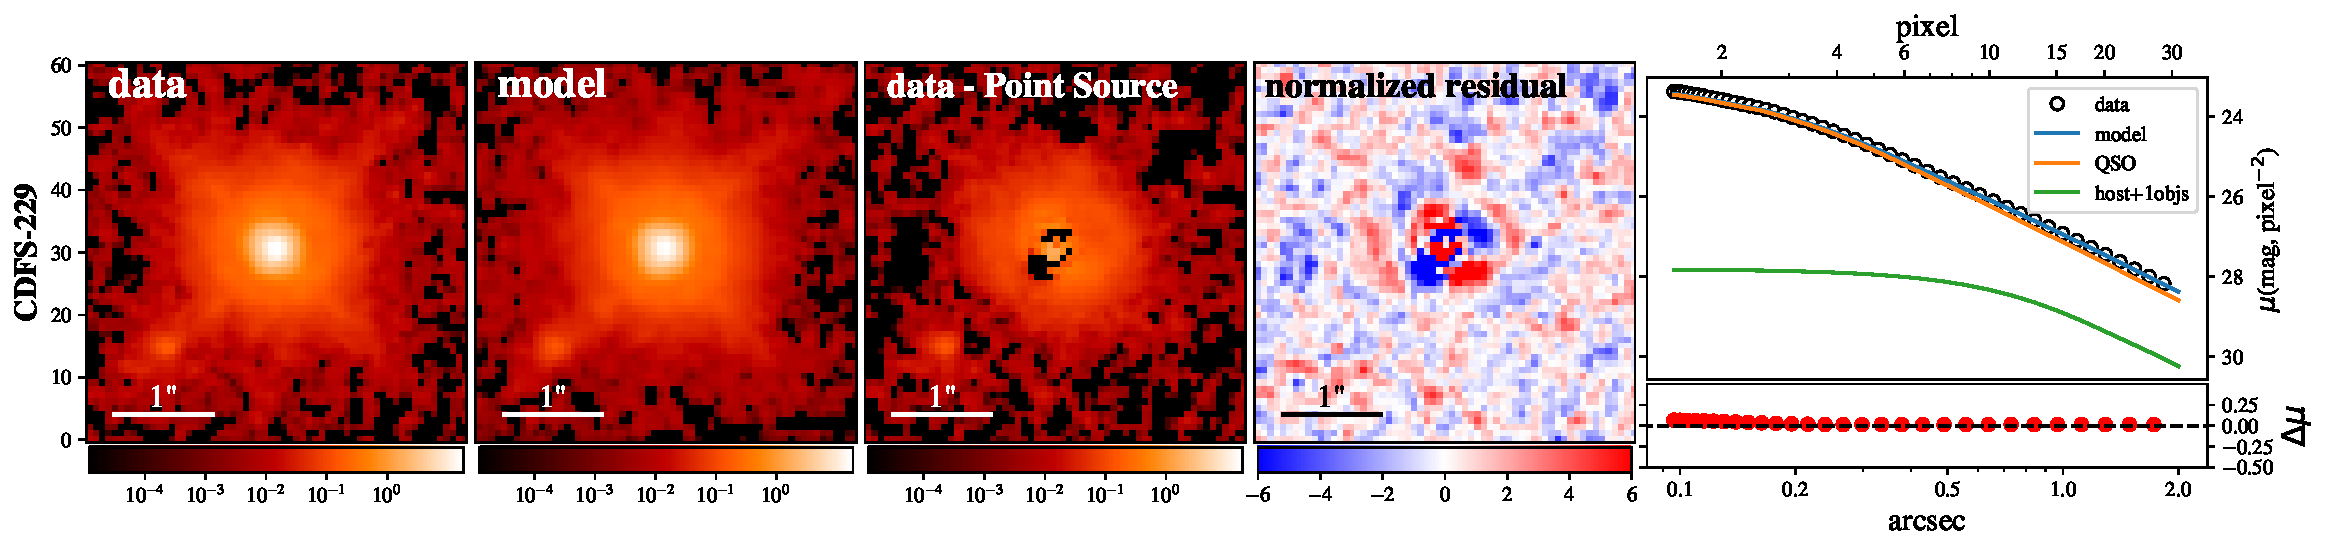
\includegraphics[height=0.25\textwidth]{fig/best_fit_CDFS-229_SB_profile.pdf}
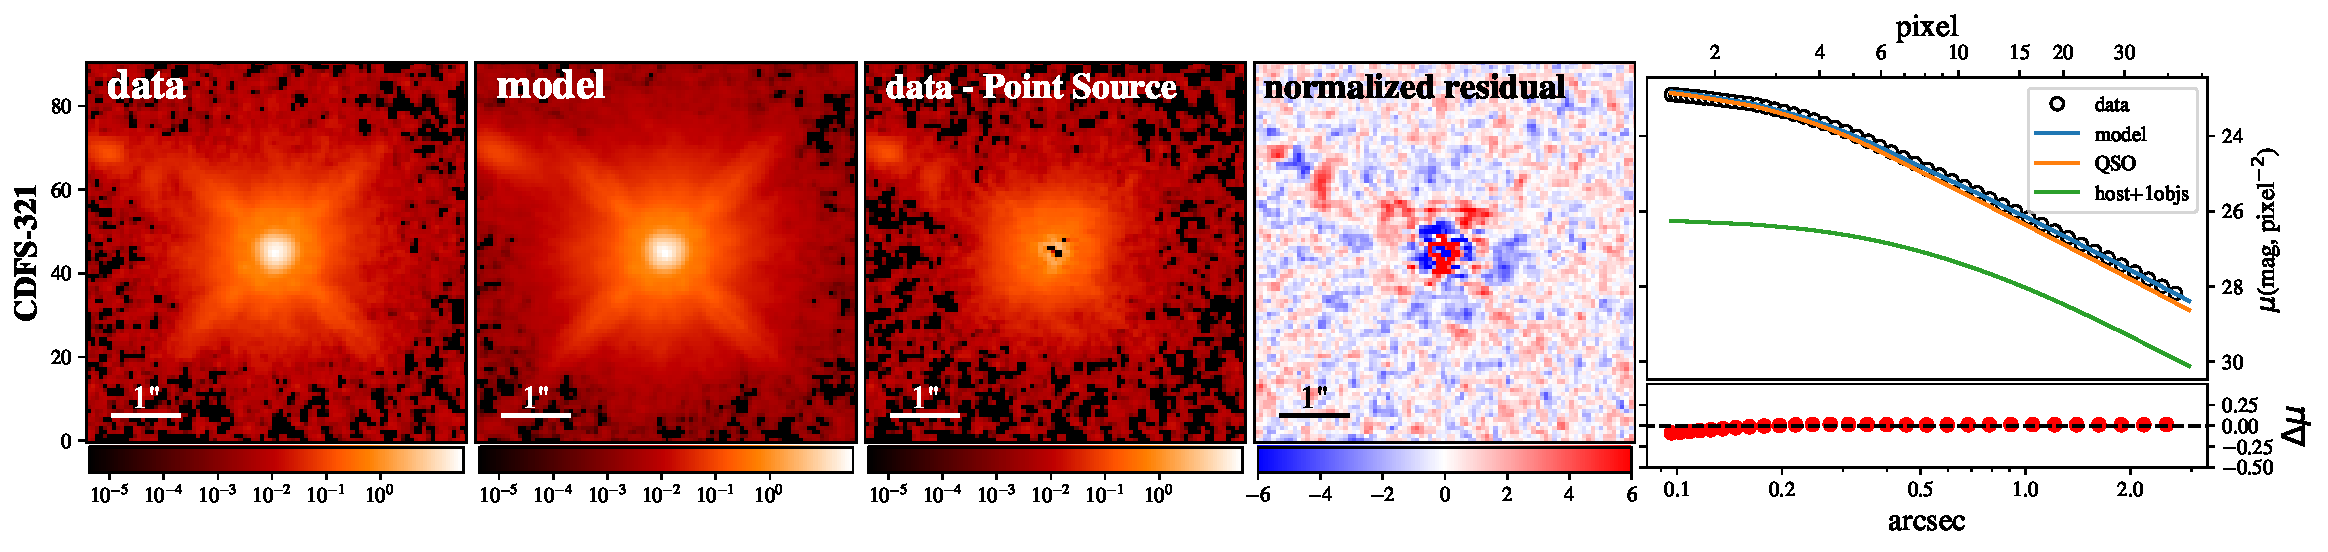
\includegraphics[height=0.25\textwidth]{fig/best_fit_CDFS-321_SB_profile.pdf}
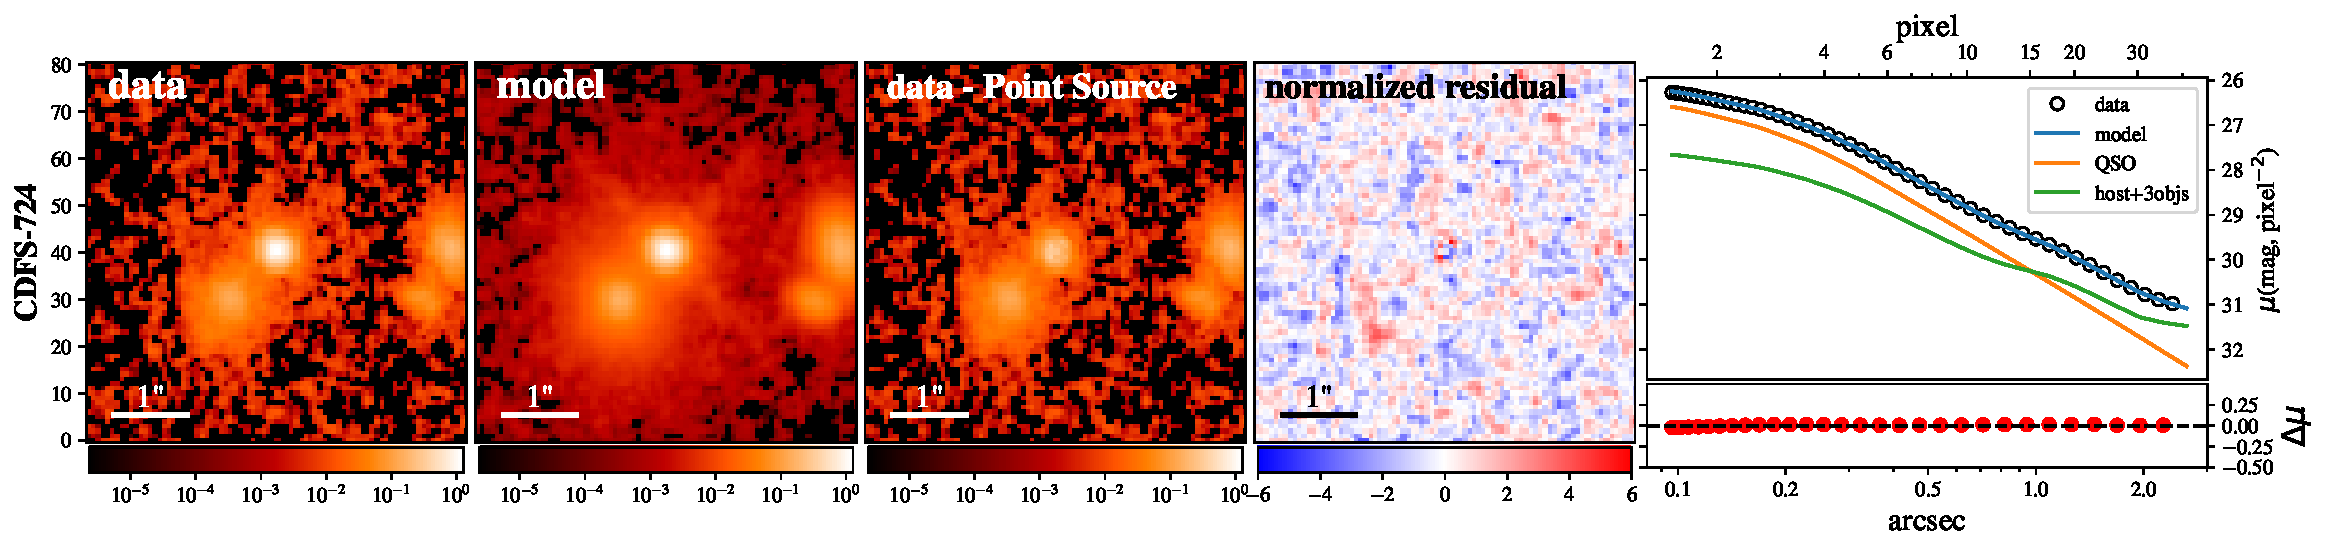
\includegraphics[height=0.25\textwidth]{fig/best_fit_CDFS-724_SB_profile.pdf}
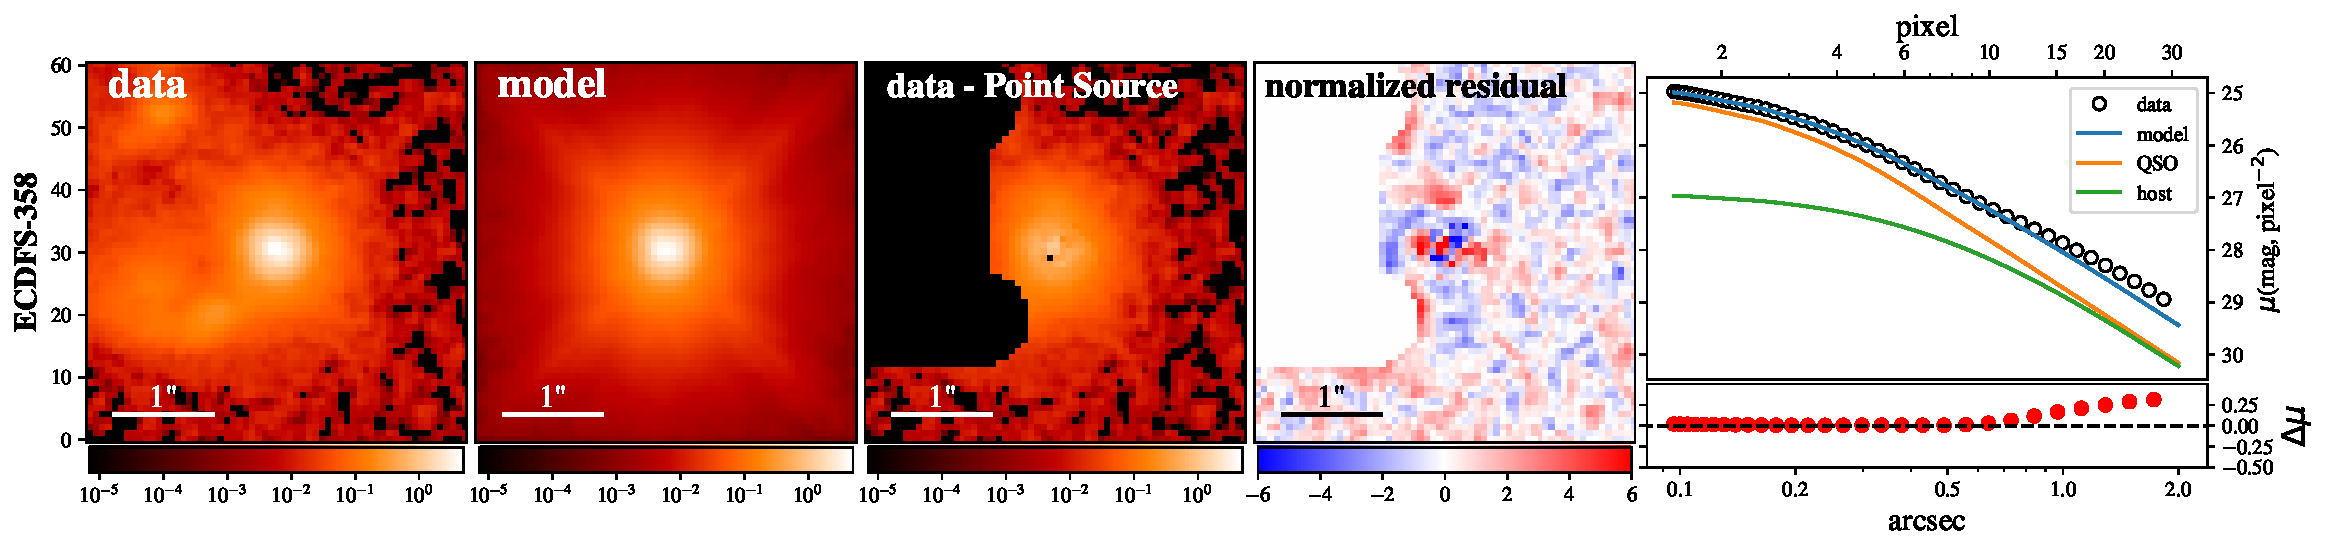
\includegraphics[height=0.25\textwidth]{fig/best_fit_ECDFS-358_SB_profile.pdf}
}
\figurenum{1}
\caption{Continued.}
\end{figure*} 

\begin{figure*}
\centering
{
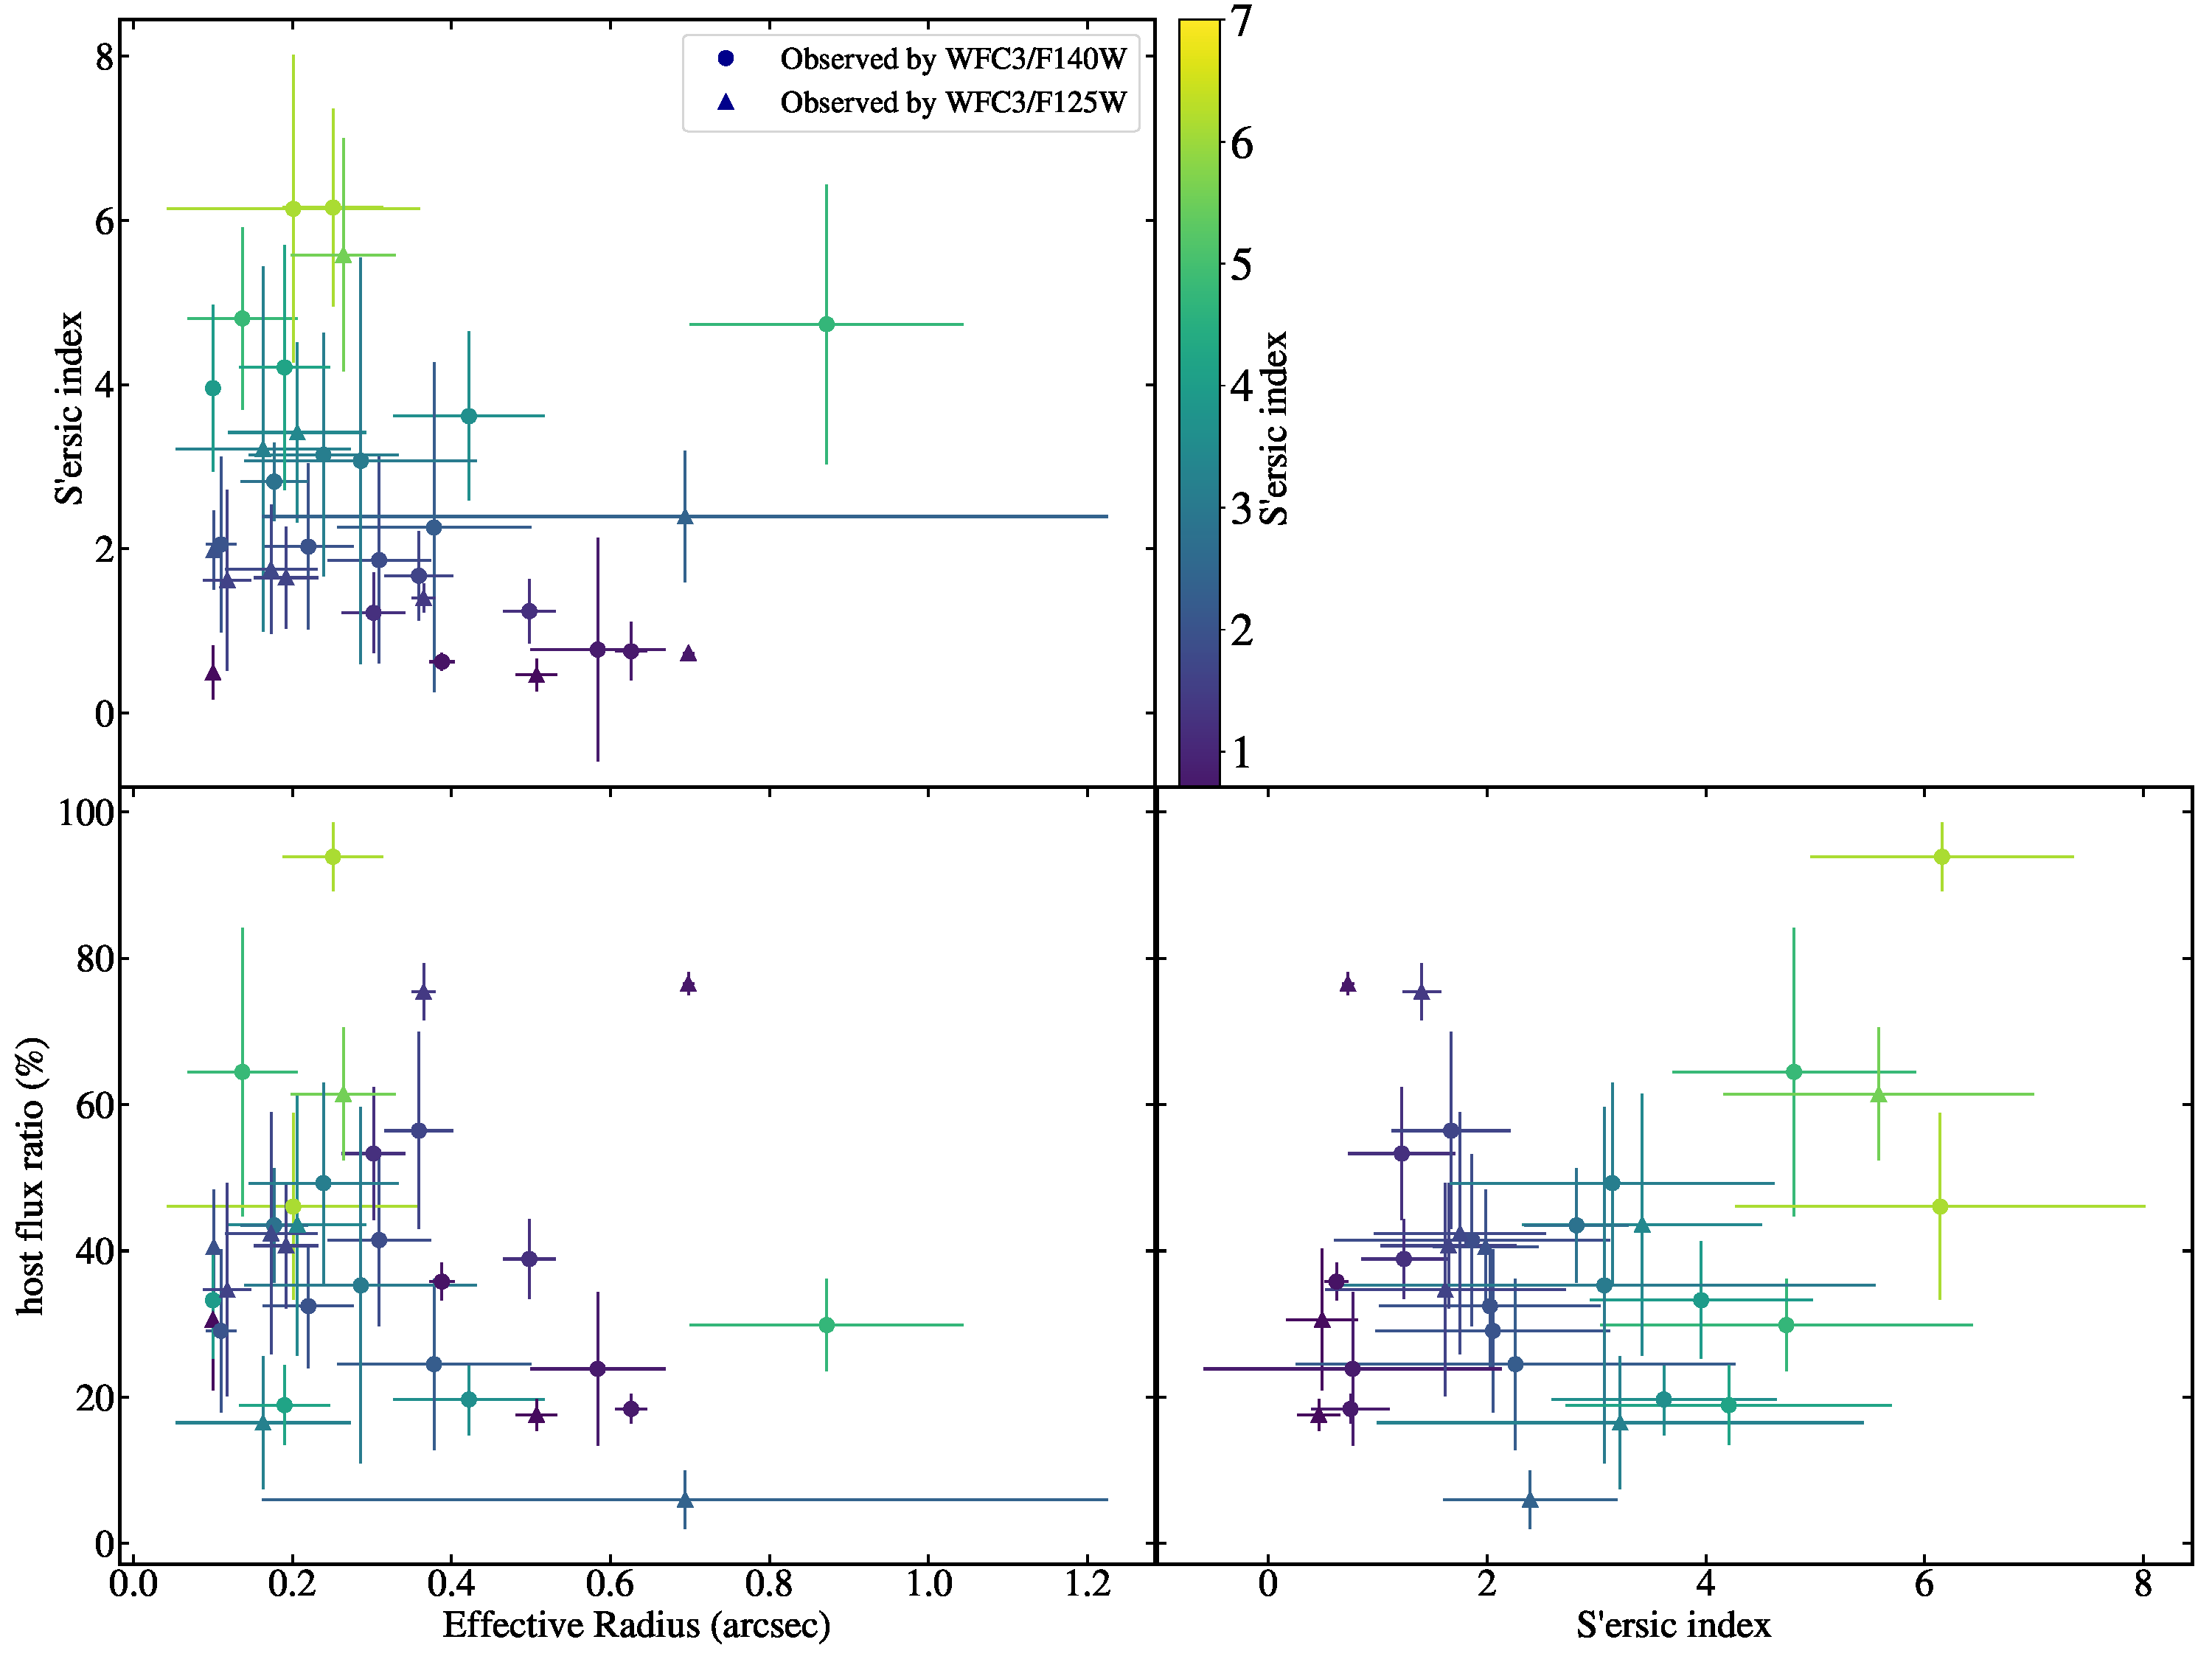
\includegraphics[height=0.75\textwidth]{fig/flux_r_n_corner.pdf}
}
\caption{\label{fig:flux_r_n_corner} The relations among these values.}
\end{figure*} 

%\appendix
%\section{If needed}
%\label{app:warp}

\end{document}